\documentclass[12pt, a4 paper]{article}
% Set target color model to RGB
\usepackage[inner=2.5cm,outer=2.5cm,top=3cm,bottom=3cm]{geometry}
\usepackage{latexsym}           % math symbols that were omitted in latex2e
\usepackage{amsbsy}             % bold greek defs
\usepackage{amsmath,graphicx}
\usepackage{bbm}
\usepackage{mathrsfs}
\usepackage{stmaryrd}
\usepackage{graphics}
\usepackage{acronym}
\usepackage{longtable}
\usepackage{mathtools}
\usepackage{setspace}
\usepackage{cite}
\usepackage{array}
\usepackage{amsmath,amsthm}
\usepackage{amssymb}
\usepackage{wasysym,url}
\usepackage{fixltx2e,amsmath}
\usepackage{setspace,float}
\usepackage{color}
\usepackage{cases,bm}
\usepackage{mathrsfs}
\usepackage{enumitem}
\usepackage{hyperref}
\usepackage{mathtools,cuted}
\usepackage[linesnumbered,ruled,vlined]{algorithm2e}
\usepackage{epsfig}
\usepackage{color}
\usepackage{sectsty}
\usepackage{subfigure}
\DontPrintSemicolon
\hypersetup{%
pdfauthor={Abijith J Kamath},%
pdftitle={Homework},%
pdfkeywords={Tikz,latex,bootstrap,uncertaintes},%
pdfcreator={PDFLaTeX},%
pdfproducer={PDFLaTeX},%
}

\newcommand{\ra}[1]{\renewcommand{\arraystretch}{#1}}

\newtheorem{thm}{Theorem}[section]
\newtheorem{prop}[thm]{Proposition}
\newtheorem{lem}[thm]{Lemma}
\newtheorem{cor}[thm]{Corollary}
\newtheorem{defn}[thm]{Definition}
\newtheorem{rem}[thm]{Remark}
\numberwithin{equation}{section}

\newcommand{\homework}[6]{
   \pagestyle{myheadings}
   \thispagestyle{plain}
   \newpage
   \setcounter{page}{1}
   \noindent
   \begin{center}
   \framebox{
      \vbox{\vspace{2mm}
    \hbox to 6.28in { {\bf E1 213:~Pattern Recognition and Neural Networks\hfill {\small Spring 2021}} }
       \vspace{6mm}
       \hbox to 6.28in { {\bfseries \Large \hfill #1  \hfill} }
       \vspace{6mm}
       \hbox to 6.28in { {\it Author: {\rm Abijith J. Kamath}} \hfill {\small {\it Email:} abijithj@iisc.ac.in}}
      \vspace{2mm}}
   }
   \end{center}
   \markboth{E1 213 -- #1}{E1 213 -- #1}
   \vspace*{4mm}
}

\newcommand{\problem}[1]{~\\\fbox{\textbf{#1}}\newline\newline}
\newcommand{\subproblem}[1]{~\newline\textbf{(#1)}}

\newcommand{\solution}{~\newline\textbf{\textit{(Solution)}} }

\linespread{1.3}

\setlength{\intextsep}{20pt} % Vertical space above & below [h] floats
\setlength{\textfloatsep}{20pt} % Vertical space below (above) [t] ([b]) floats
\setlength{\abovecaptionskip}{10pt}
\setlength{\belowcaptionskip}{10pt}

\newcommand{\by}{\mathbf{y}}
\newcommand{\bx}{\mathbf{x}}
\newcommand{\bX}{\mathbf{X}}
\newcommand{\bW}{\mathbf{W}}
\newcommand{\bA}{\mathbf{A}}
\newcommand{\bF}{\mathbf{F}}
\newcommand{\rr}{\mathbb{R}}
\newcommand{\cc}{\mathbb{C}}
\newcommand{\Ex}{\mathbb{E}}
\newcommand{\TT}{\mathsf{T}}
\newcommand{\HH}{\mathsf{H}}

\newcommand{\bmu}{\boldsymbol{\mu}}
\newcommand{\btheta}{\boldsymbol{\theta}}
\newcommand{\bSigma}{\boldsymbol{\Sigma}}

\chapterfont{\fontfamily{lmss}\selectfont}
\sectionfont{\fontfamily{lmss}\selectfont}
\subsectionfont{\fontfamily{lmss}\selectfont}

\begin{document}
\homework{Assignment 3: Non-Linear Models}{}






% ------------------------------------------------------------------------------------------------------------------------------------------------------

\section{SVM for Classification on 2D Synthetic Data}
\label{sec:svm_synthetic}

The classification task is to classify $2$D features in two classes. Support vector machines (SVM) with polynomial and Gaussian kernel are used classification along with logistic regression for comparison.

{\it \bfseries Results:} Figure \ref{fig:LS_LOG_Gamma} shows the accuracies of classification in confusion matrices and the samples along with the discriminant function. The first and third columns shows the confusion matrices of the linear classifier and logistic regression, respectively with varying training sizes. The second and fourth column shows the samples along with the discriminant function. The accuracies reported are averaged over $10000$ realisations and one of the discriminant functions is plotted. \\

\begin{figure}
\centering
\subfigure[Poly, Size $500$]{\label{fig:a}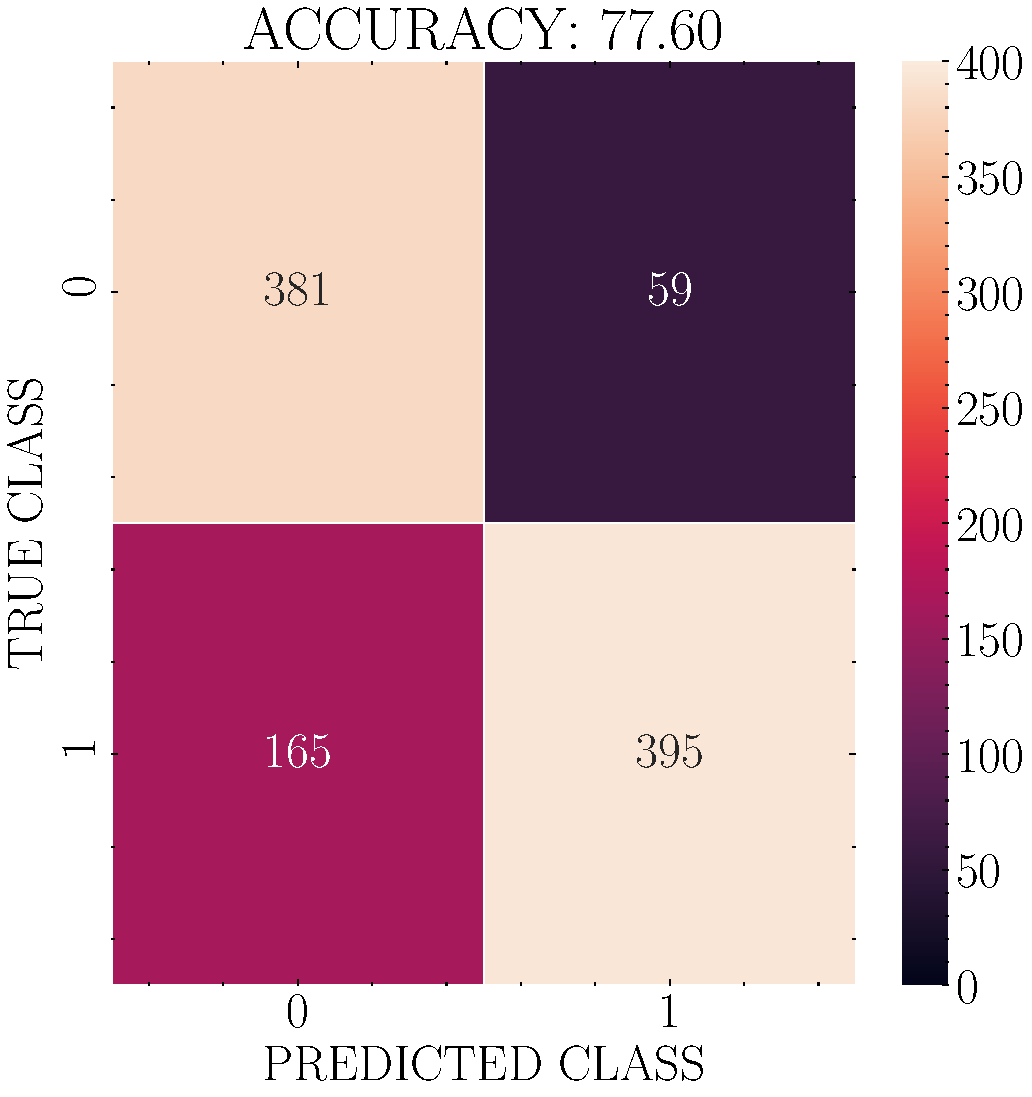
\includegraphics[width=1.5in]{../results/ex1/accuracy_SVM_dataset_noise0_method_poly_size_500}}
\subfigure[SVM-Poly, Classifier]{\label{fig:a}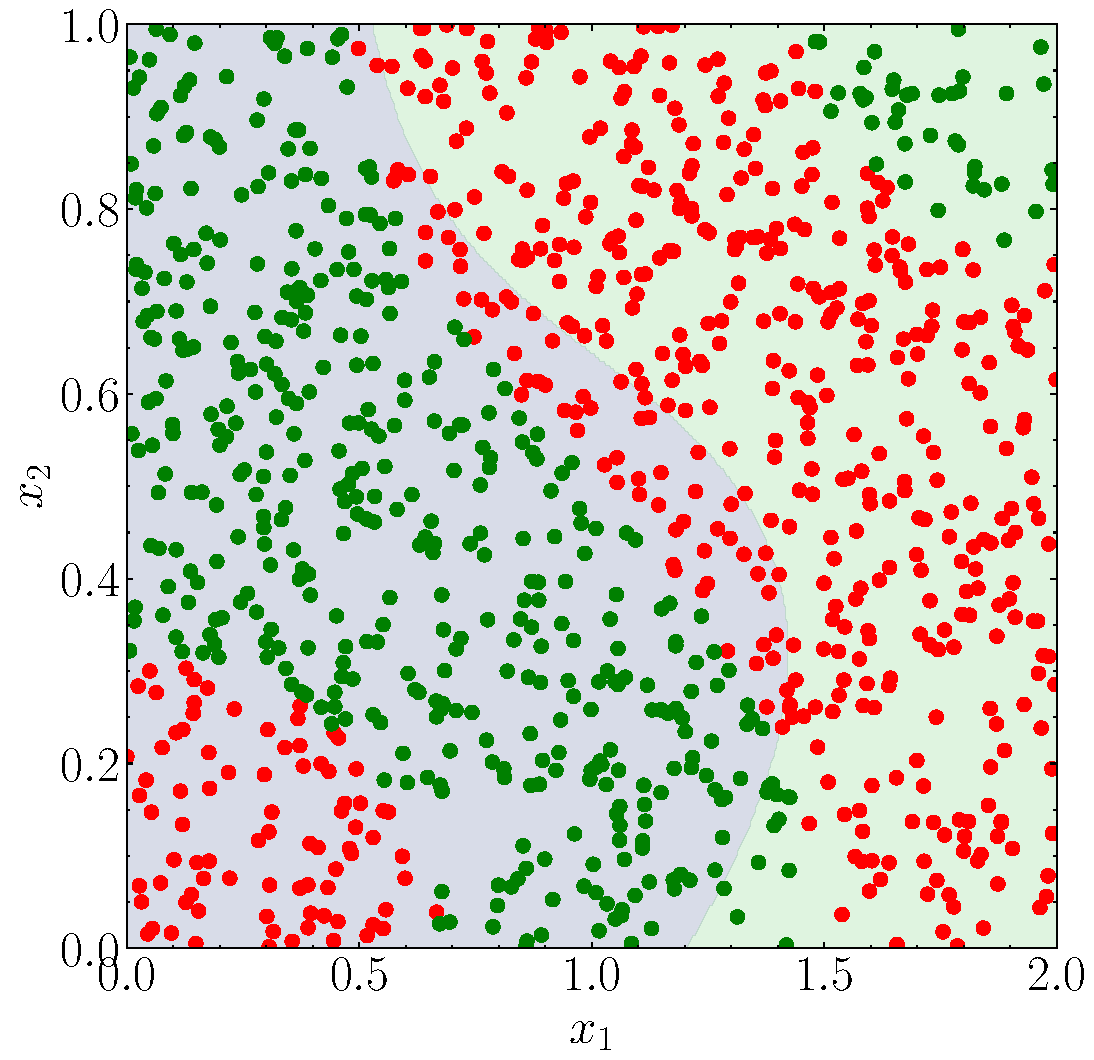
\includegraphics[width=1.5in]{../results/ex1/samples_SVM_dataset_noise0_method_poly_size_500}}
\subfigure[RBF, Size $500$]{\label{fig:a}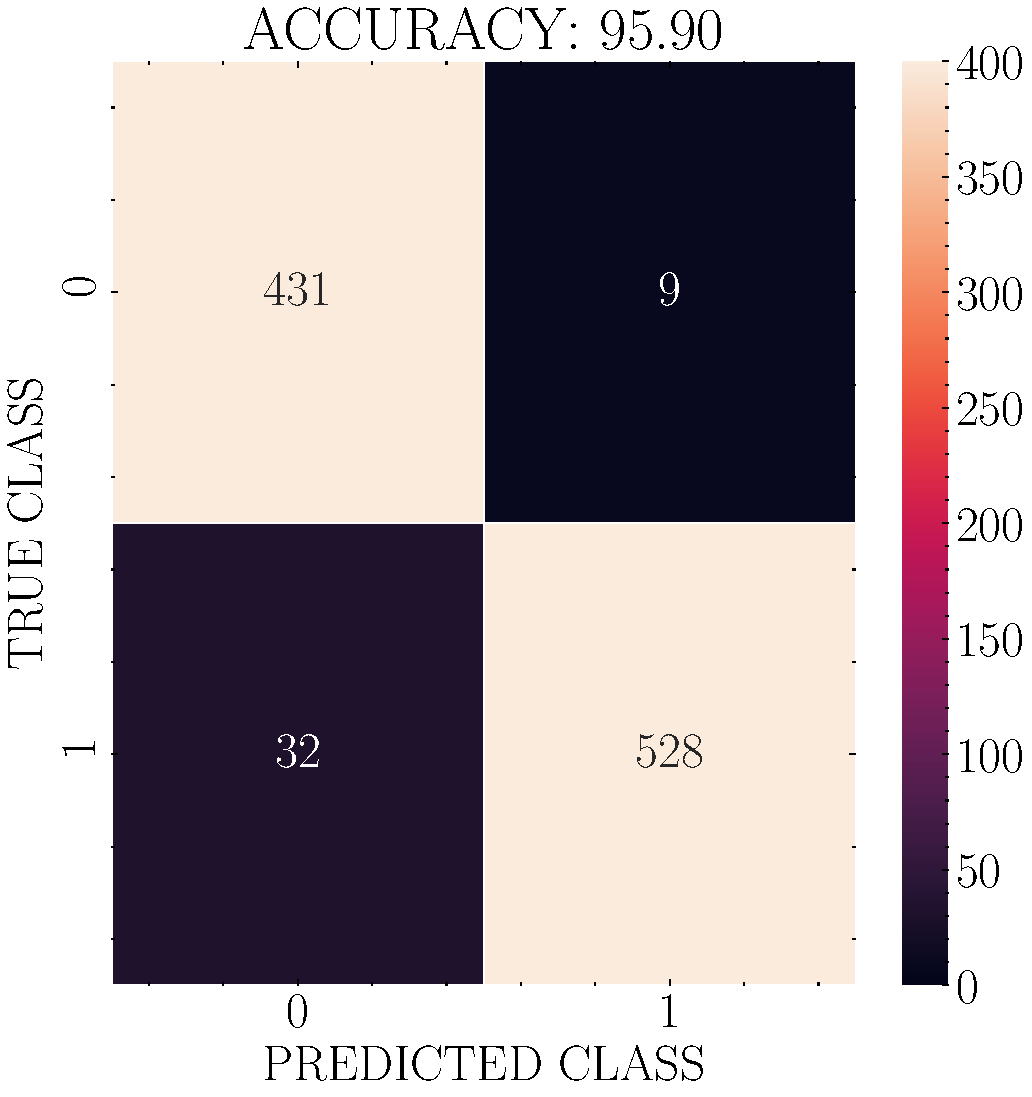
\includegraphics[width=1.5in]{../results/ex1/accuracy_SVM_dataset_noise0_method_rbf_size_500}}
\subfigure[SVM-RBF Classifier]{\label{fig:a}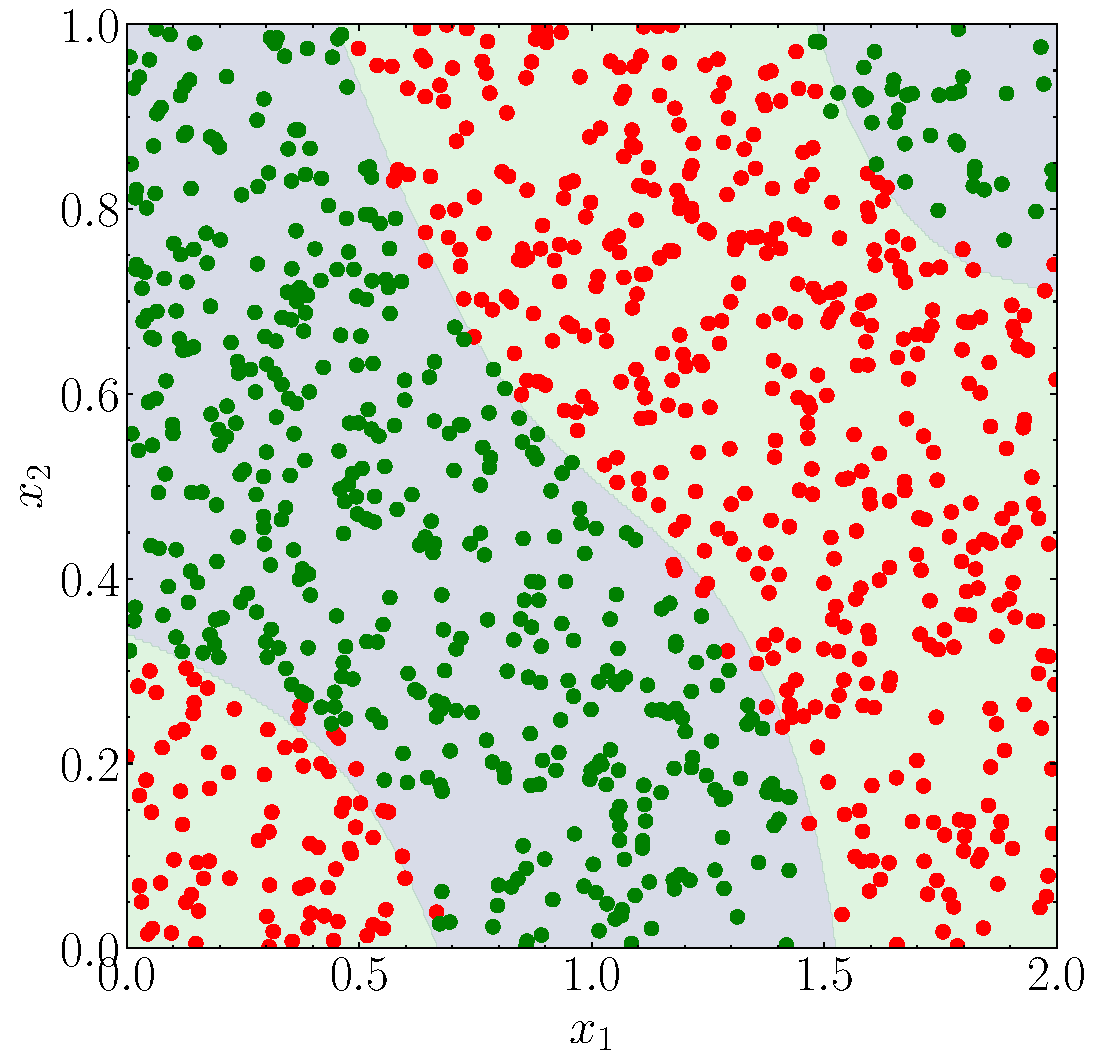
\includegraphics[width=1.5in]{../results/ex1/samples_SVM_dataset_noise0_method_rbf_size_500}}

\subfigure[Poly, Size $1000$]{\label{fig:a}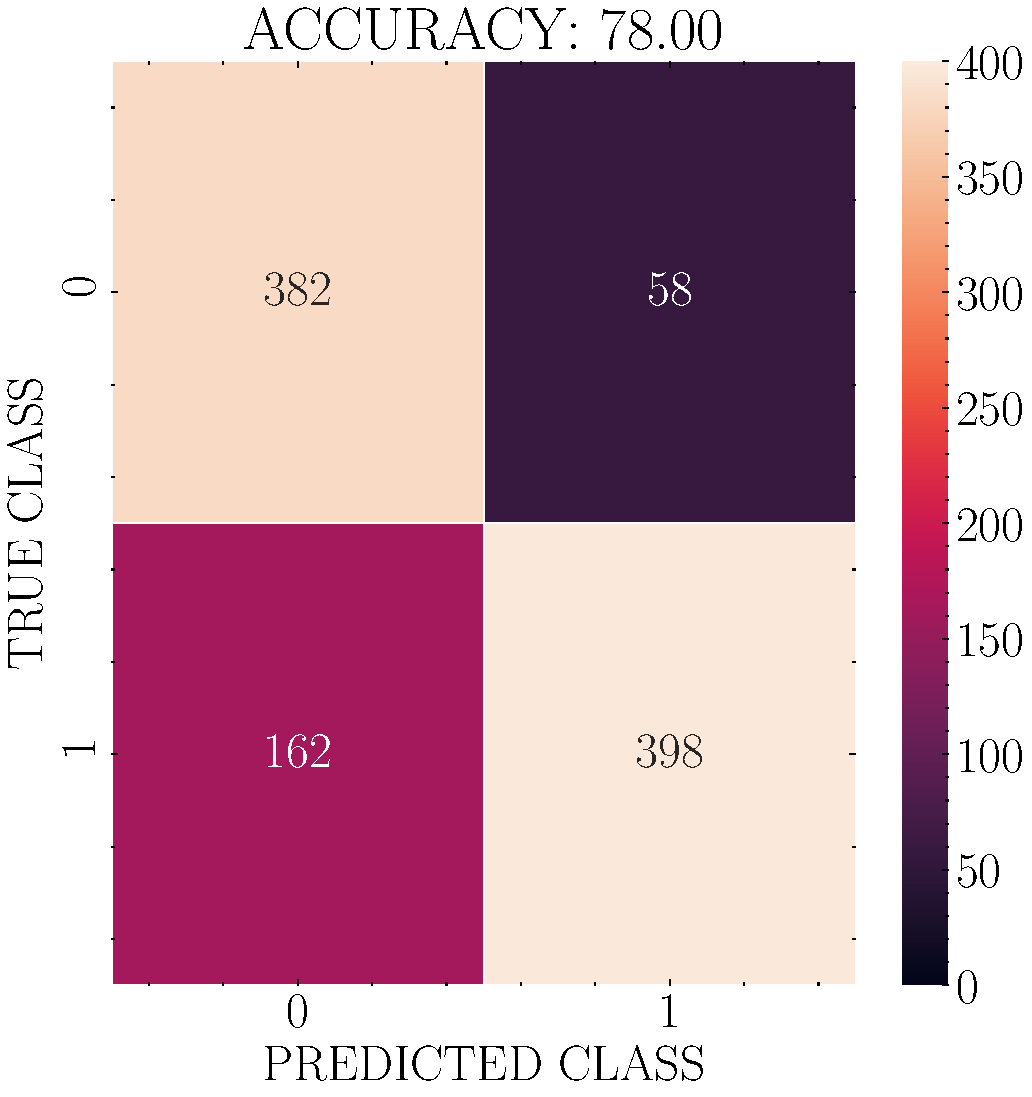
\includegraphics[width=1.5in]{../results/ex1/accuracy_SVM_dataset_noise0_method_poly_size_1000}}
\subfigure[SVM-Poly, Classifier]{\label{fig:a}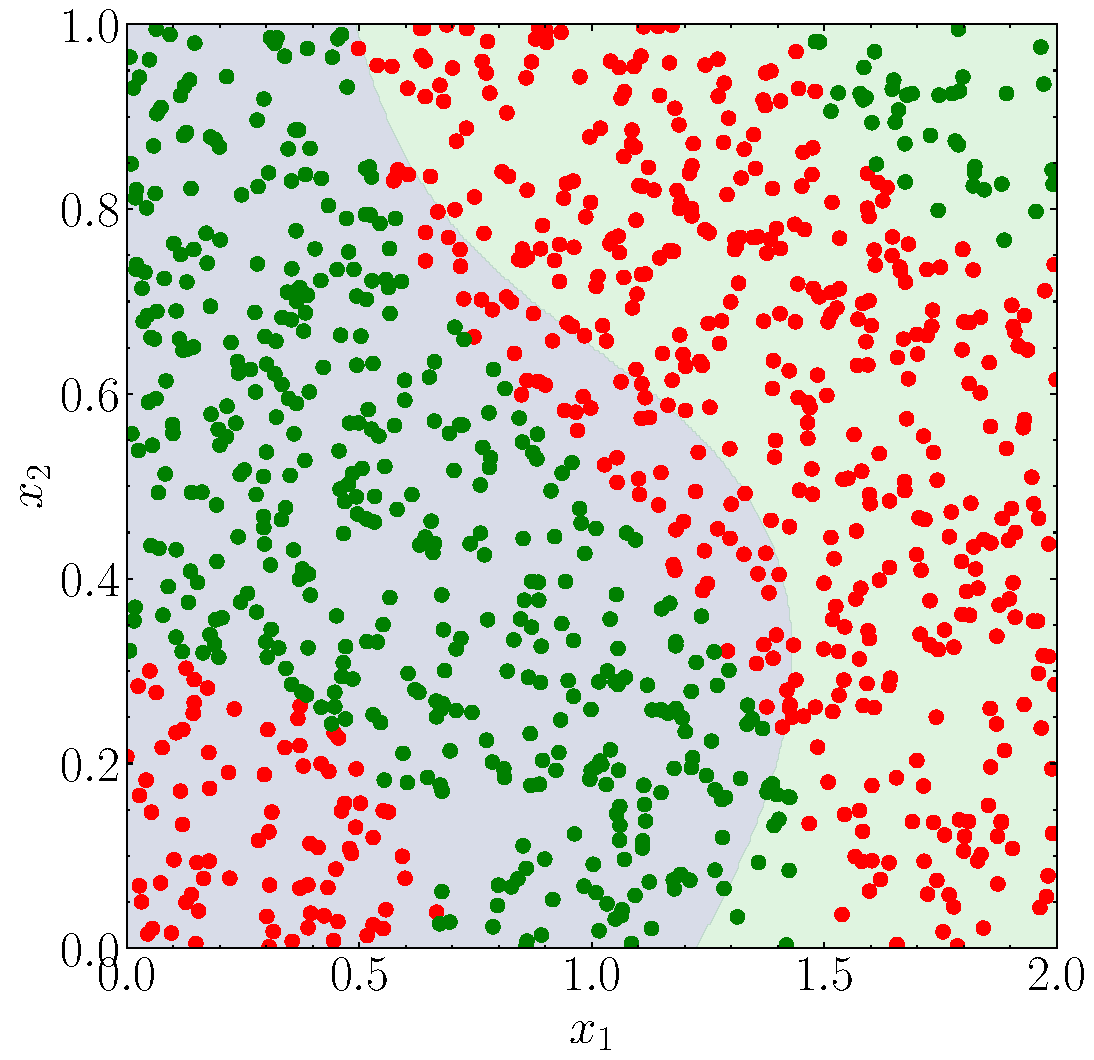
\includegraphics[width=1.5in]{../results/ex1/samples_SVM_dataset_noise0_method_poly_size_1000}}
\subfigure[RBF, Size $1000$]{\label{fig:a}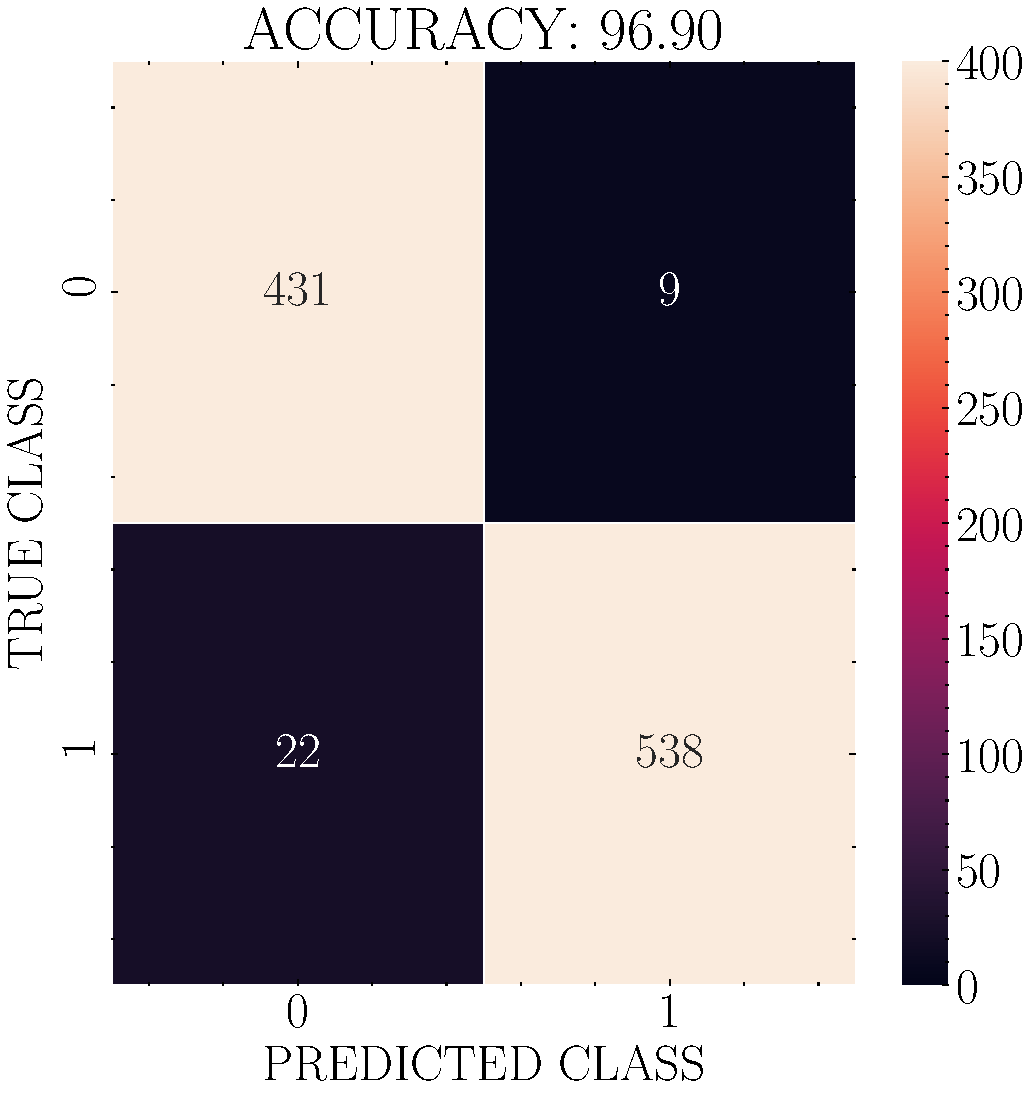
\includegraphics[width=1.5in]{../results/ex1/accuracy_SVM_dataset_noise0_method_rbf_size_1000}}
\subfigure[SVM-RBF Classifier]{\label{fig:a}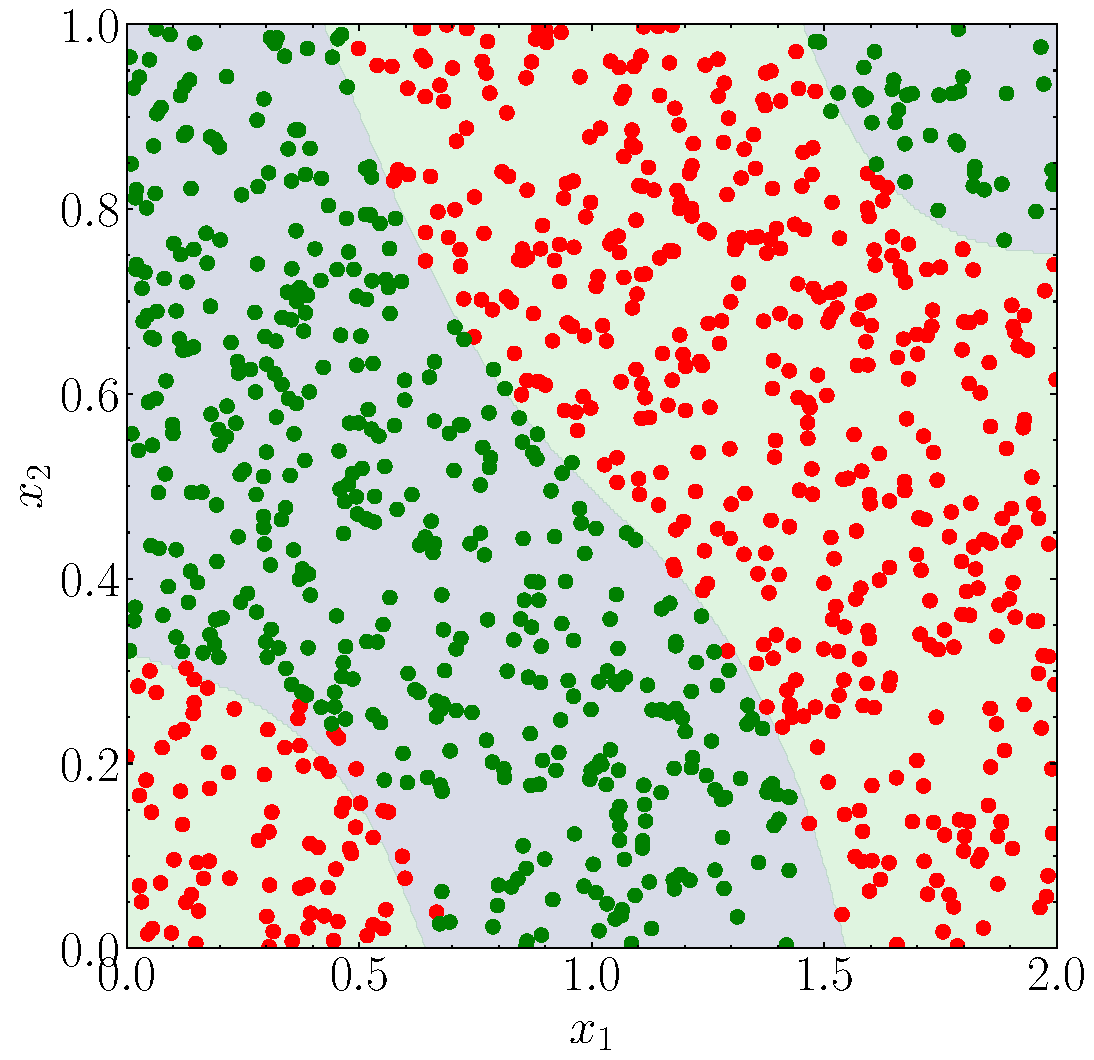
\includegraphics[width=1.5in]{../results/ex1/samples_SVM_dataset_noise0_method_rbf_size_1000}}

\subfigure[Poly, Size $1500$]{\label{fig:a}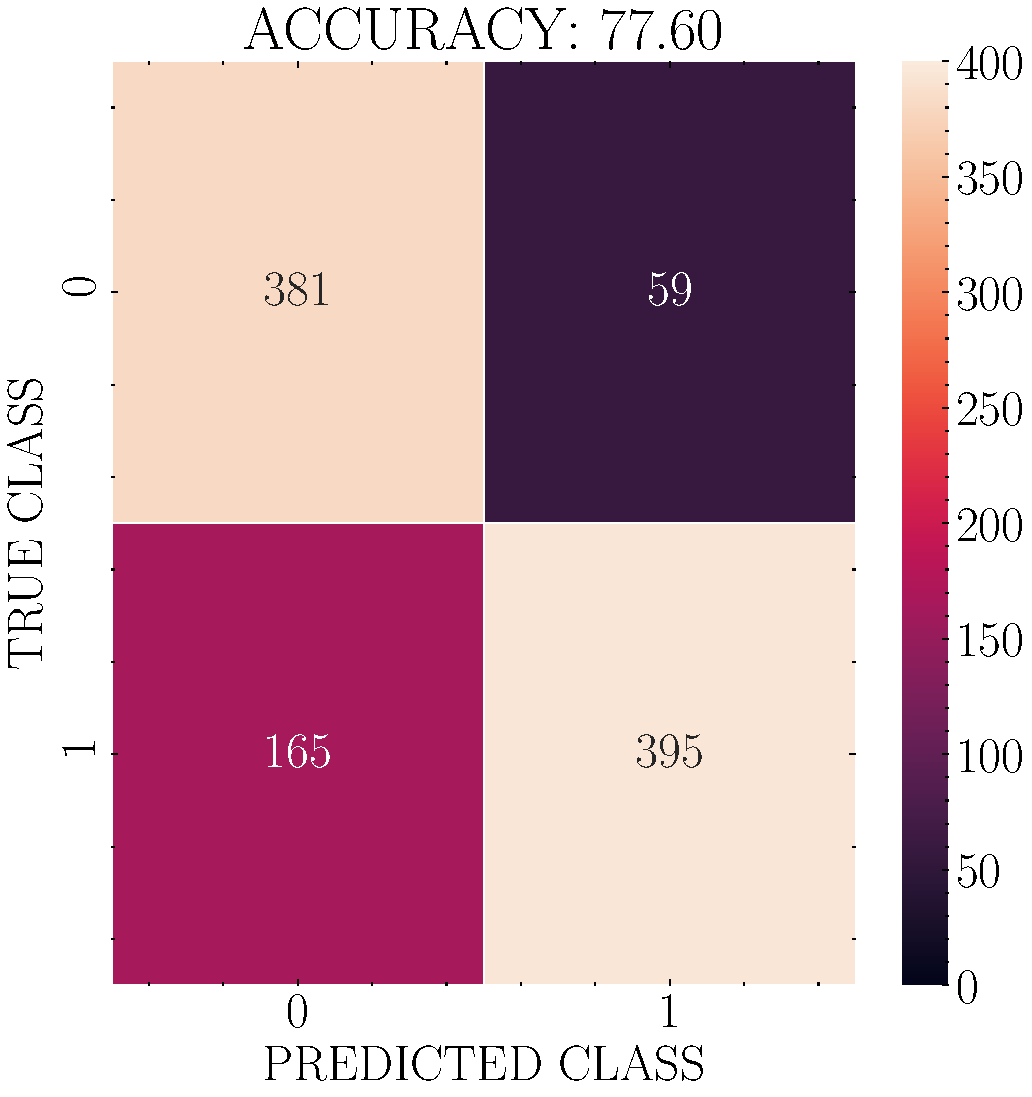
\includegraphics[width=1.5in]{../results/ex1/accuracy_SVM_dataset_noise0_method_poly_size_1500}}
\subfigure[SVM-Poly, Classifier]{\label{fig:a}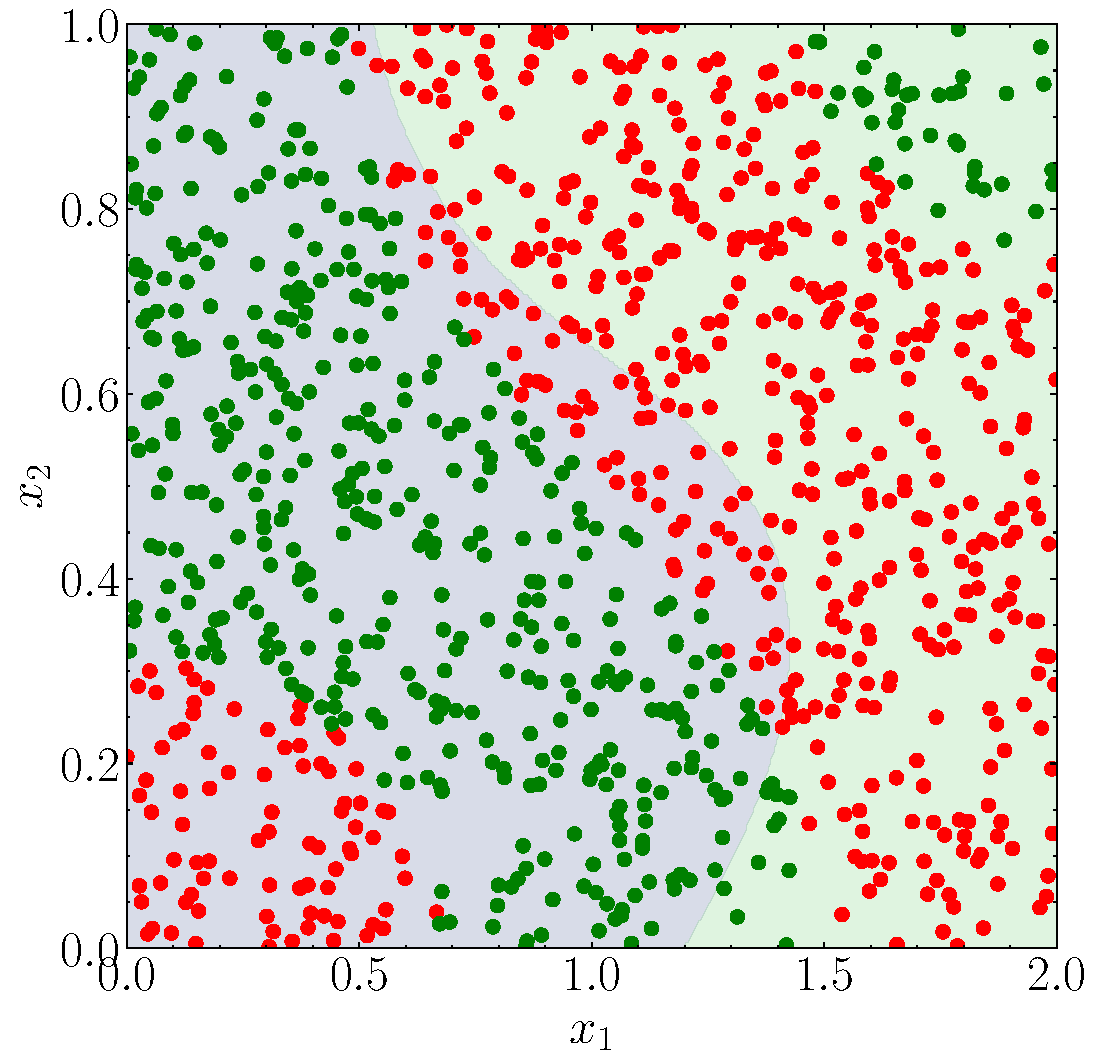
\includegraphics[width=1.5in]{../results/ex1/samples_SVM_dataset_noise0_method_poly_size_1500}}
\subfigure[RBF, Size $1500$]{\label{fig:a}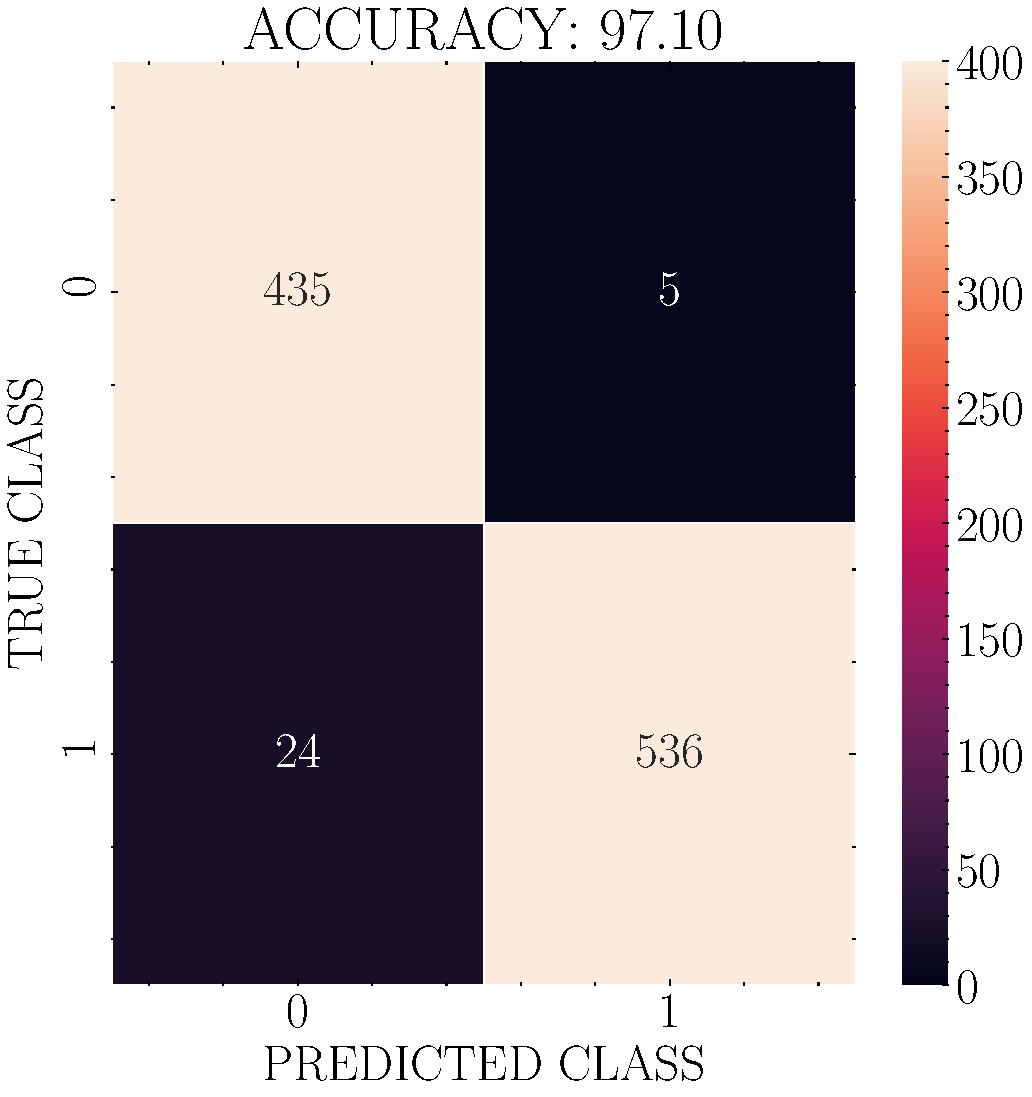
\includegraphics[width=1.5in]{../results/ex1/accuracy_SVM_dataset_noise0_method_rbf_size_1500}}
\subfigure[SVM-RBF Classifier]{\label{fig:a}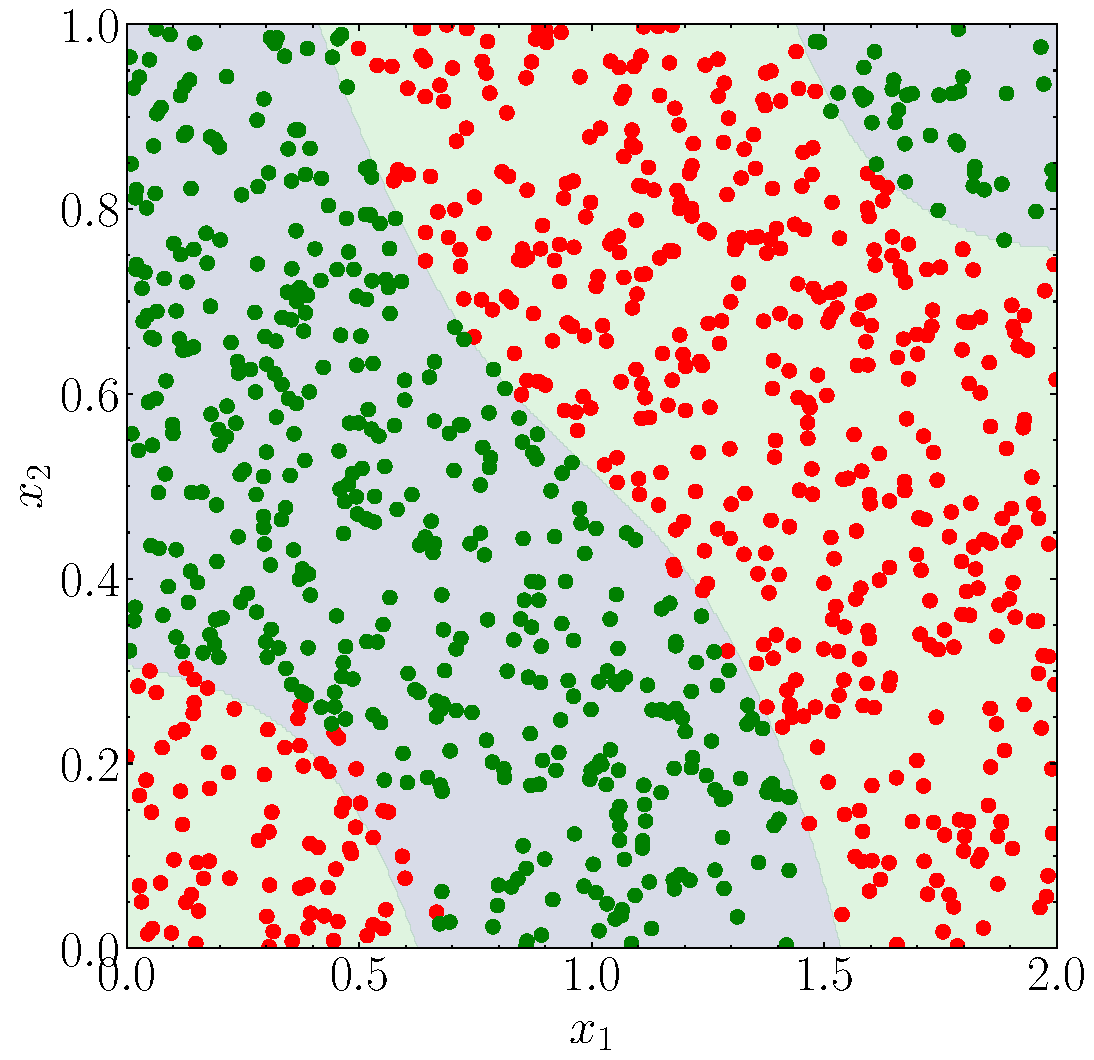
\includegraphics[width=1.5in]{../results/ex1/samples_SVM_dataset_noise0_method_rbf_size_1500}}

\subfigure[Poly, Size $2000$]{\label{fig:a}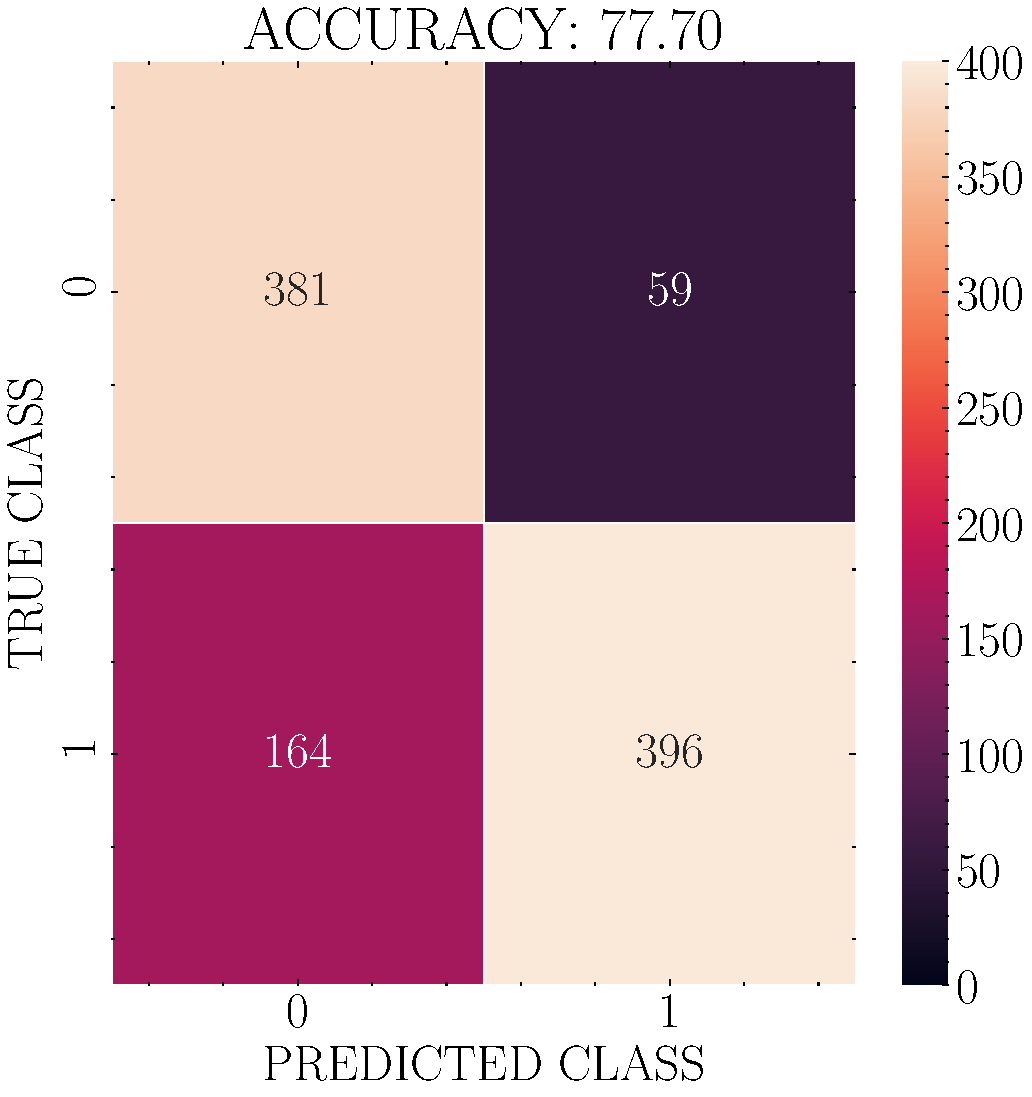
\includegraphics[width=1.5in]{../results/ex1/accuracy_SVM_dataset_noise0_method_poly_size_2000}}
\subfigure[SVM-Poly, Classifier]{\label{fig:a}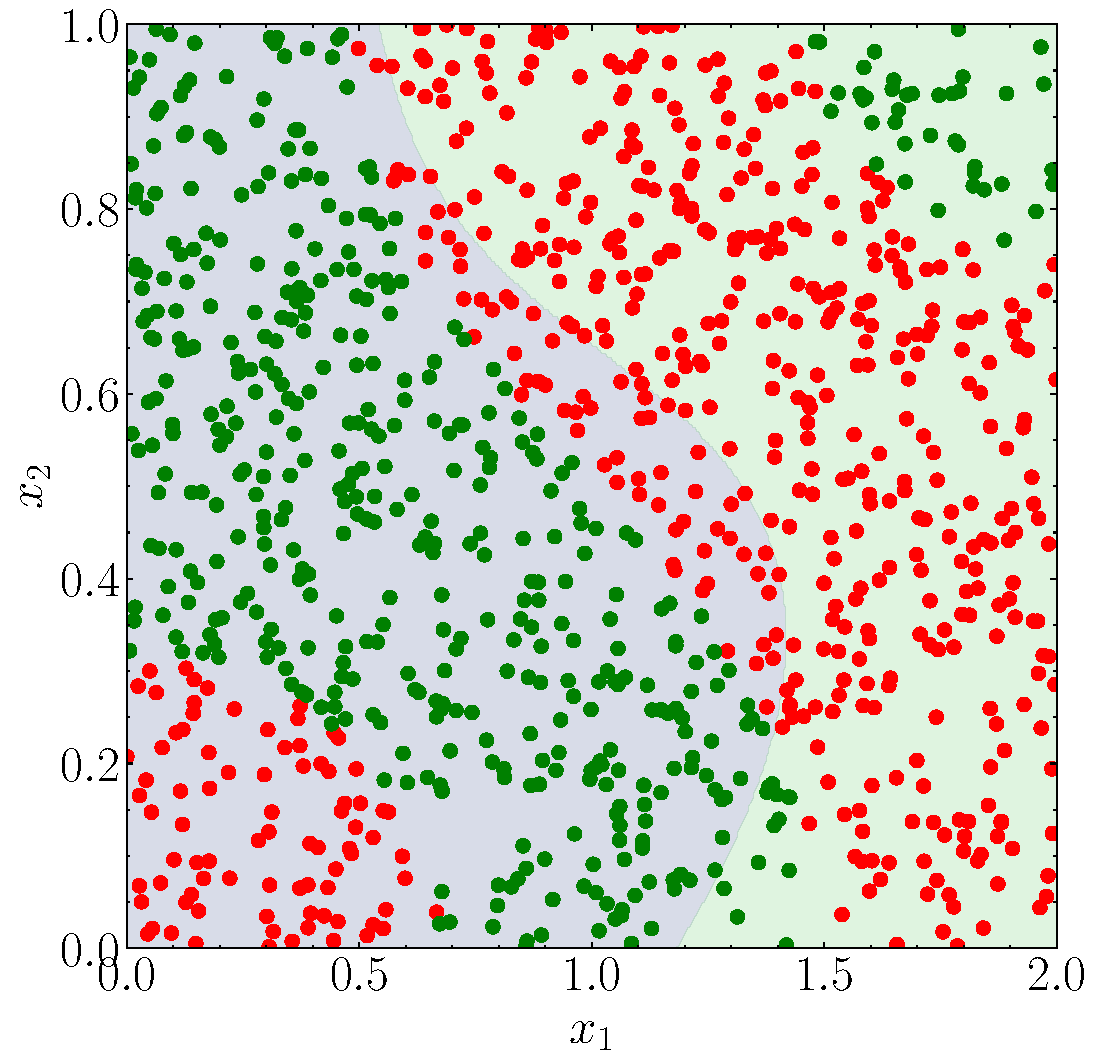
\includegraphics[width=1.5in]{../results/ex1/samples_SVM_dataset_noise0_method_poly_size_2000}}
\subfigure[RBF, Size $2000$]{\label{fig:a}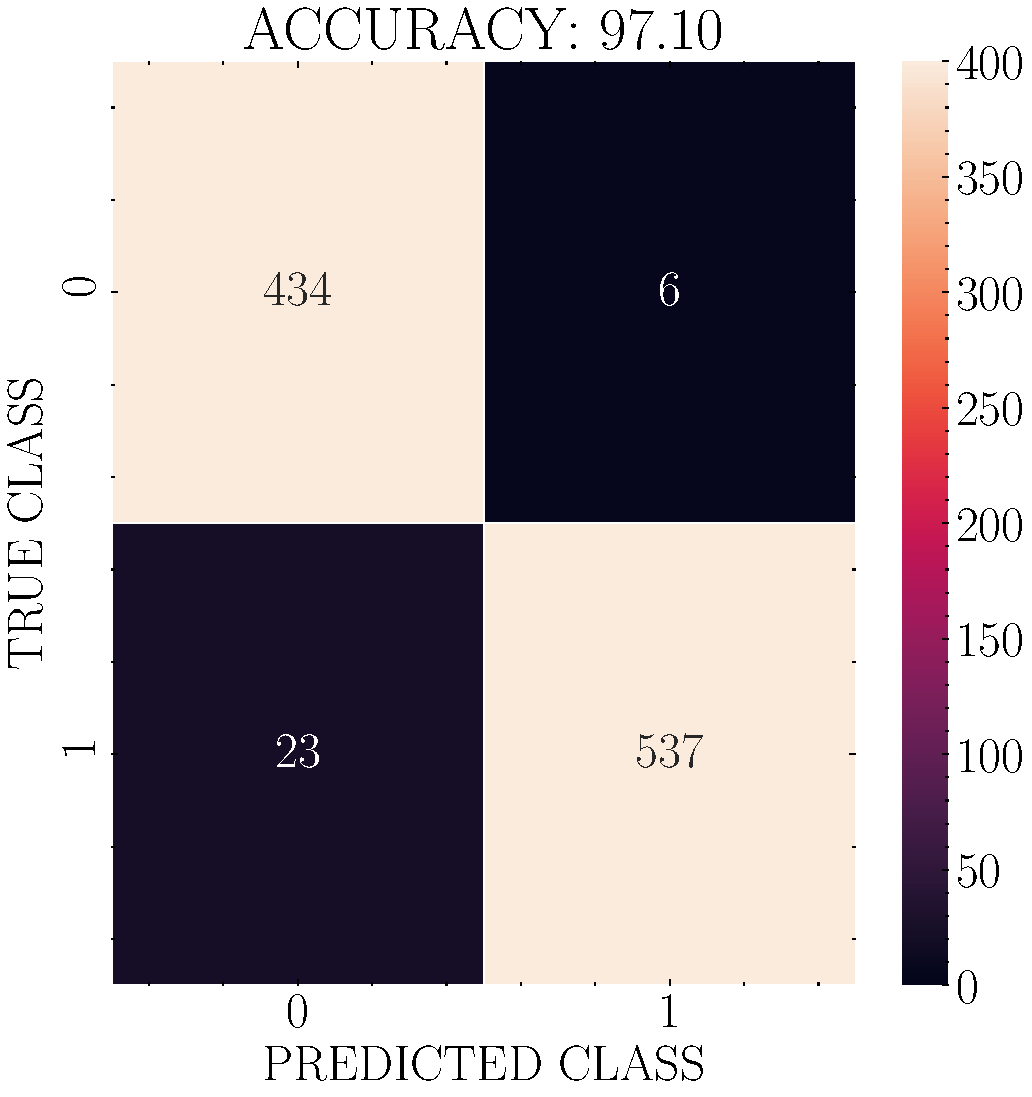
\includegraphics[width=1.5in]{../results/ex1/accuracy_SVM_dataset_noise0_method_rbf_size_2000}}
\subfigure[SVM-RBF Classifier]{\label{fig:a}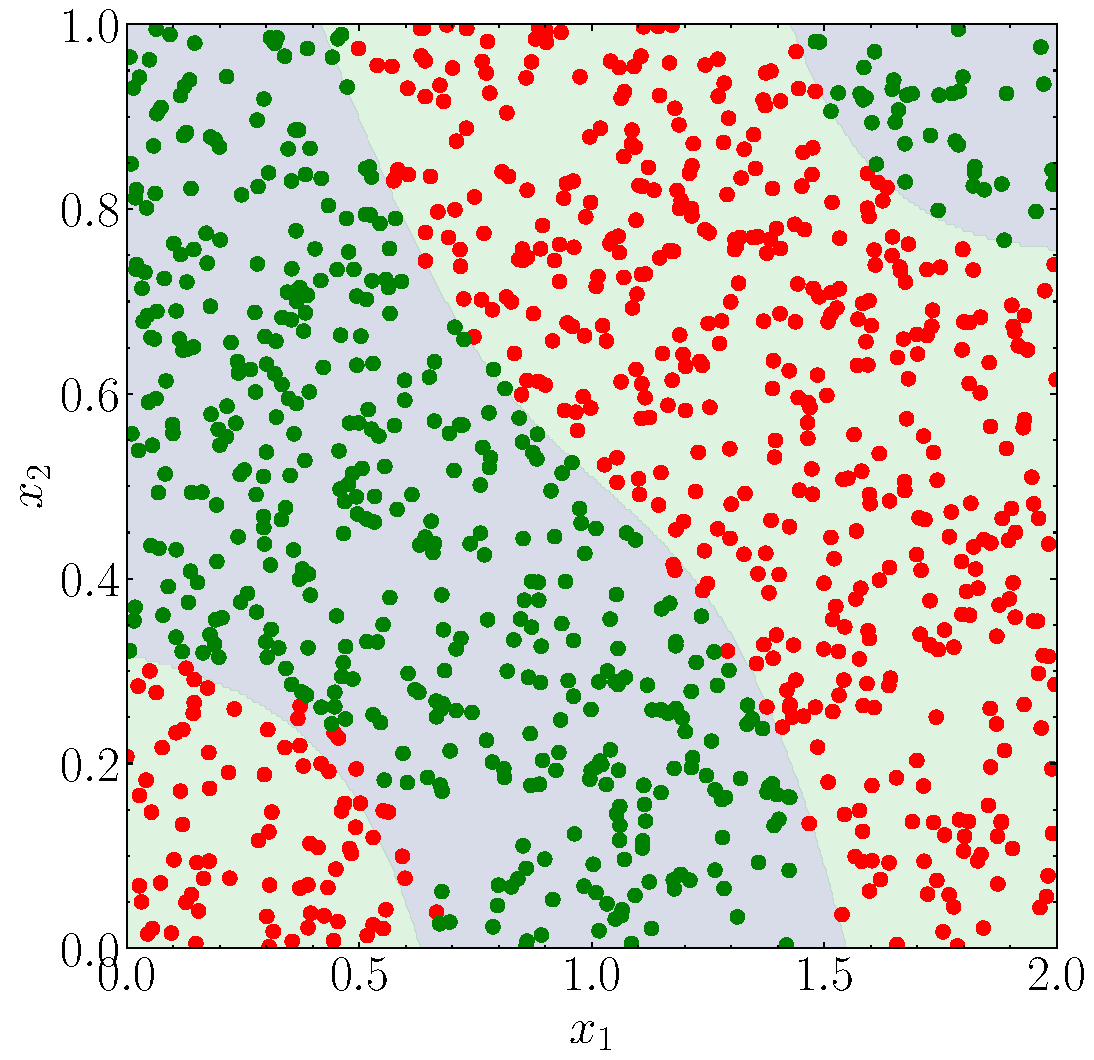
\includegraphics[width=1.5in]{../results/ex1/samples_SVM_dataset_noise0_method_rbf_size_2000}}

\caption{Support vector machines with polynomial kernel of degree $3$ and Gaussian kernel on 2D data with no label noise.}
\label{fig:SVM_ex1_noise0}
\end{figure}

\begin{figure}
\centering
\subfigure[Poly, Size $500$]{\label{fig:a}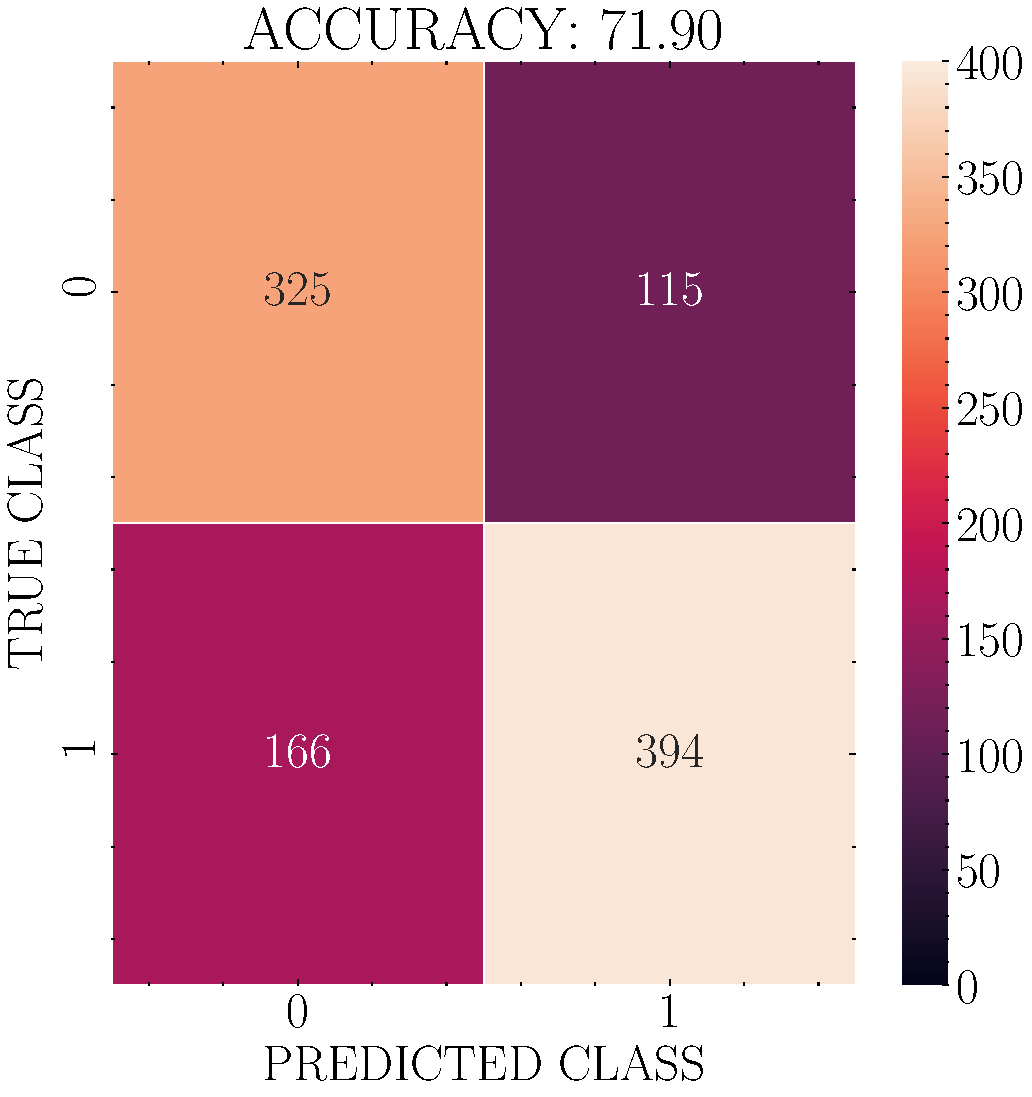
\includegraphics[width=1.5in]{../results/ex1/accuracy_LOG_dataset_noise0_size_500}}
\subfigure[Poly, Size $1000$]{\label{fig:a}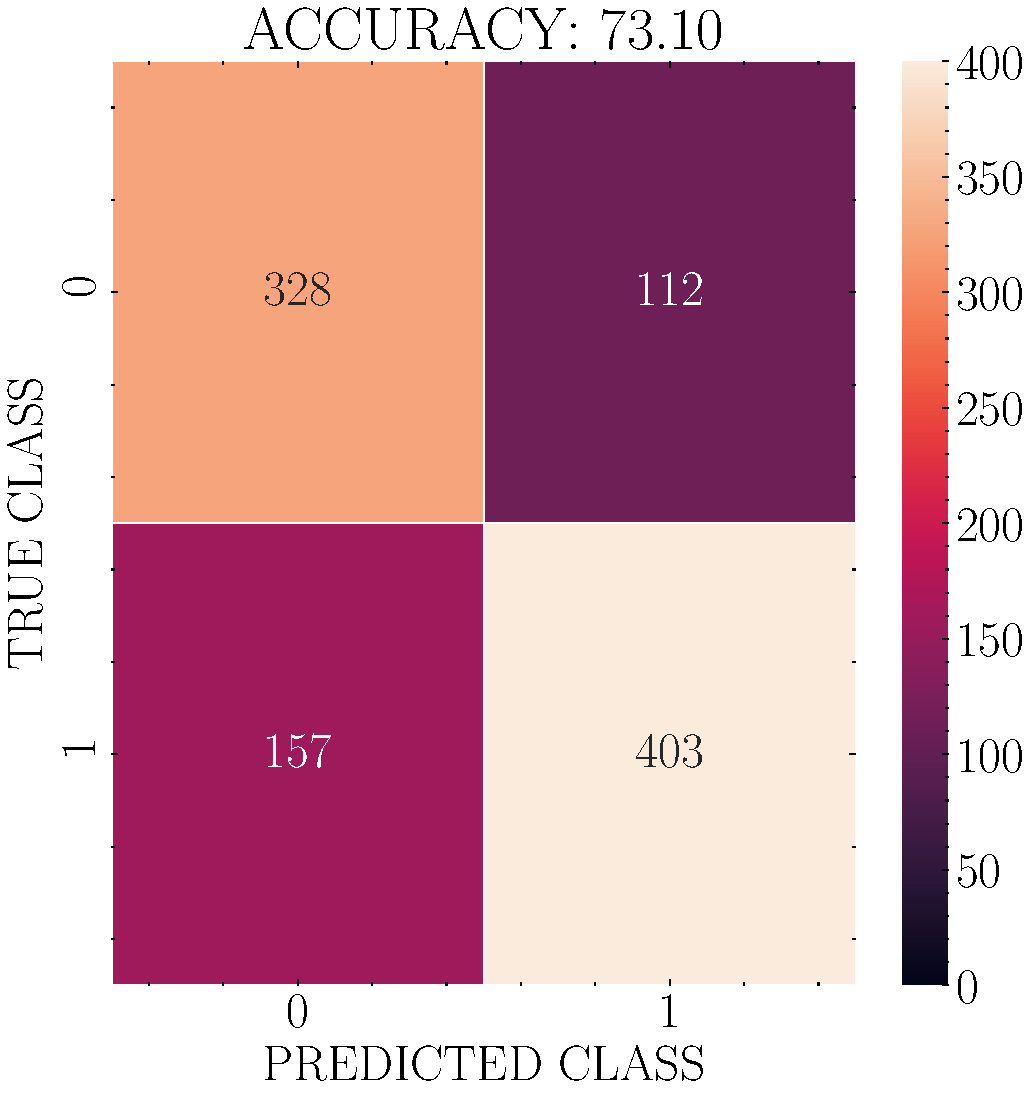
\includegraphics[width=1.5in]{../results/ex1/accuracy_LOG_dataset_noise0_size_1000}}
\subfigure[Poly, Size $1500$]{\label{fig:a}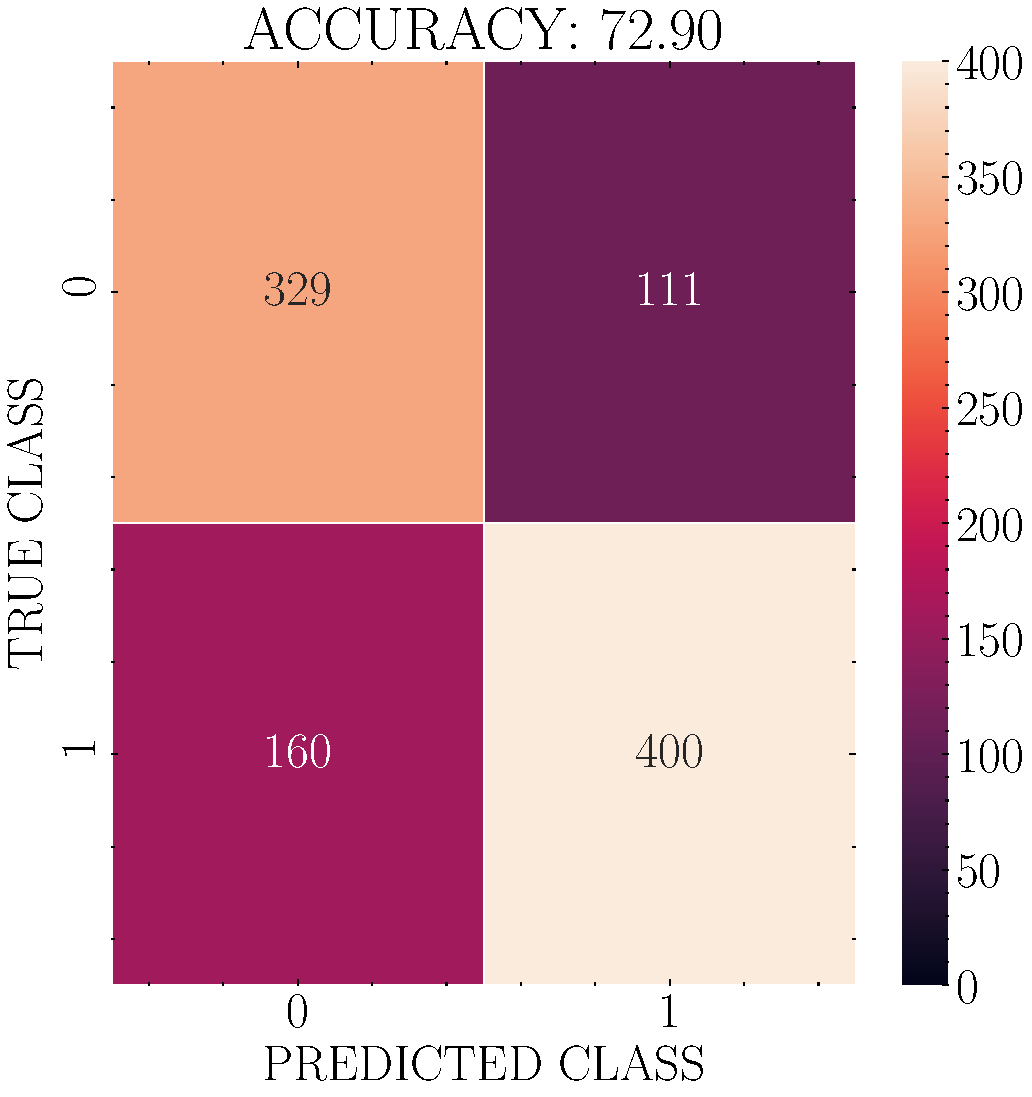
\includegraphics[width=1.5in]{../results/ex1/accuracy_LOG_dataset_noise0_size_1500}}
\subfigure[Poly, Size $2000$]{\label{fig:a}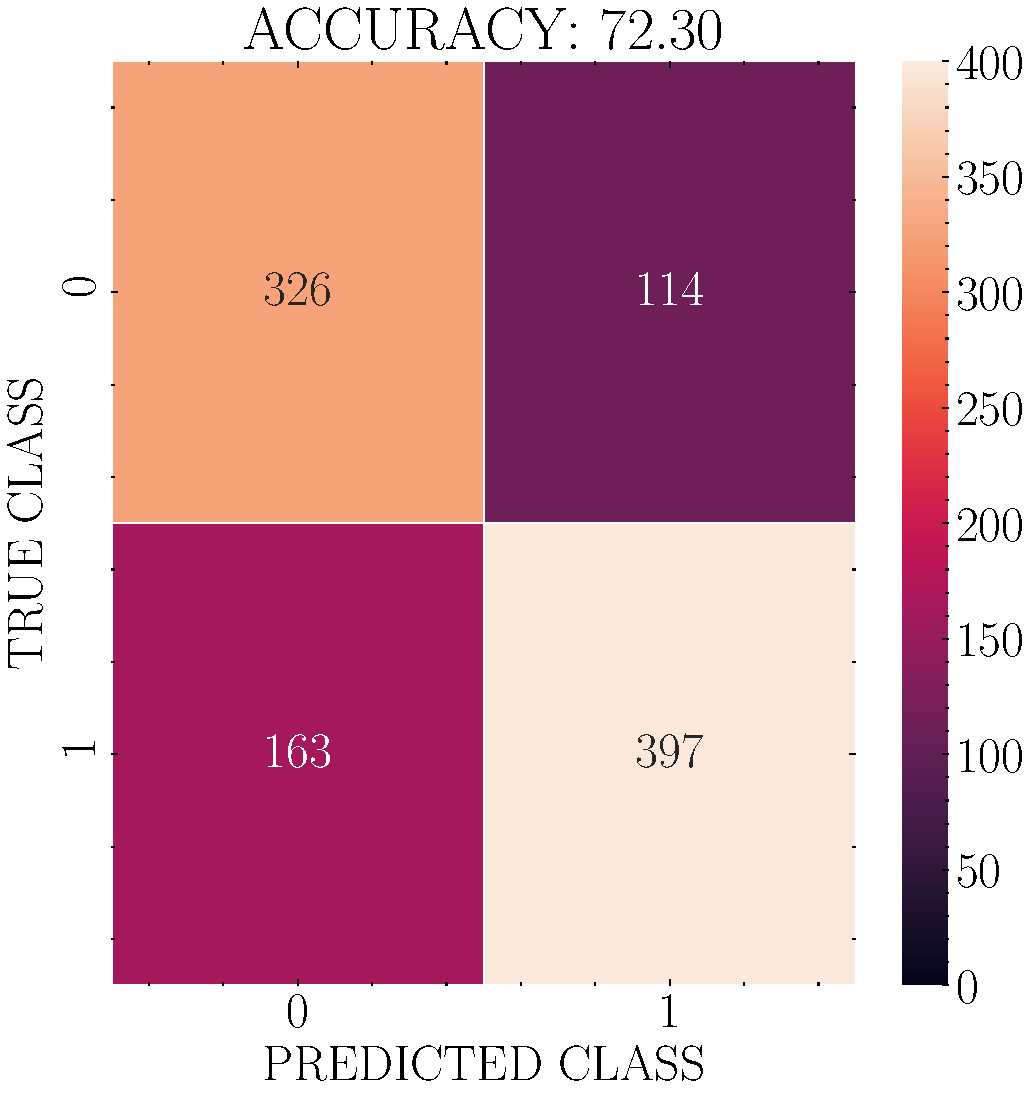
\includegraphics[width=1.5in]{../results/ex1/accuracy_LOG_dataset_noise0_size_2000}}

\subfigure[LOG, Classifier]{\label{fig:a}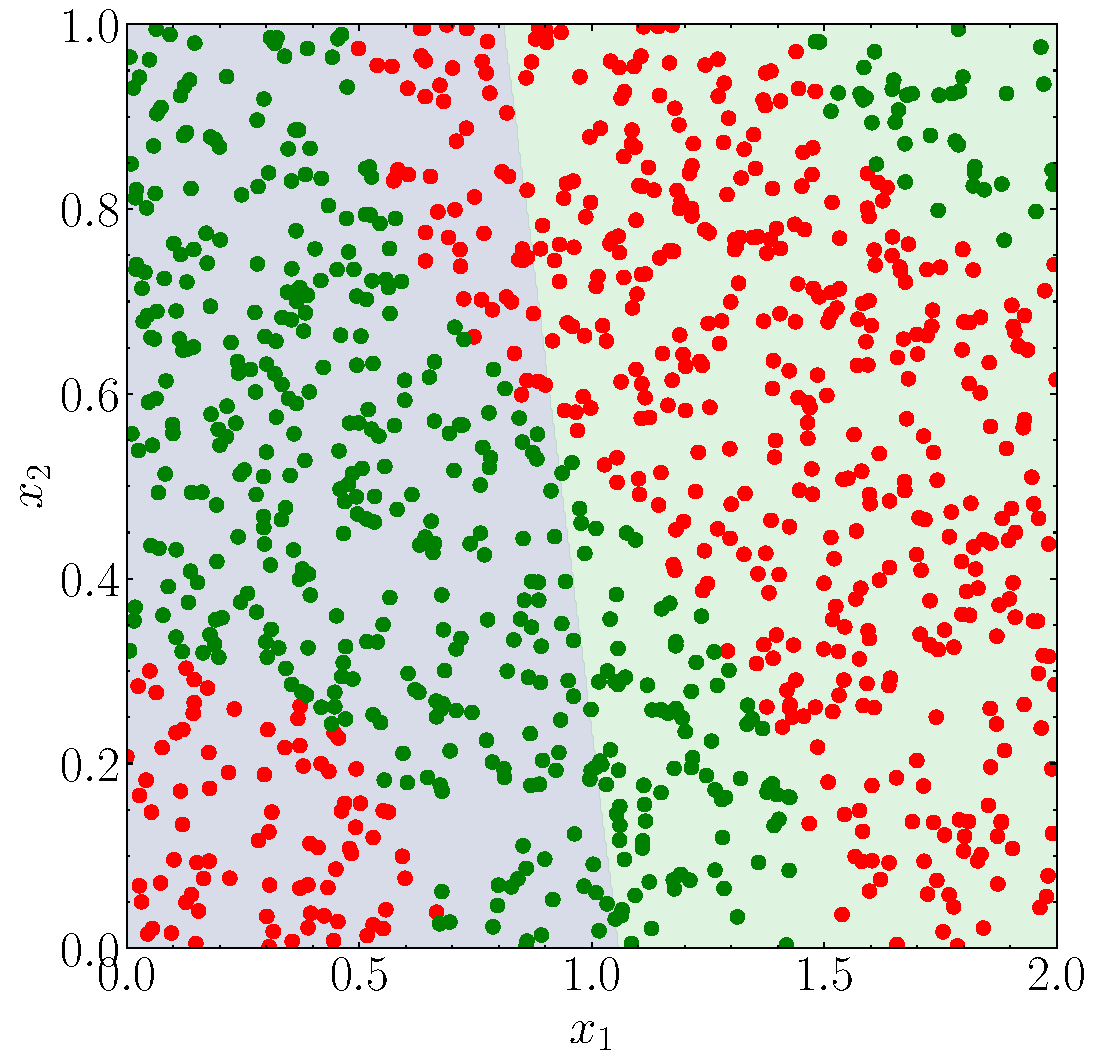
\includegraphics[width=1.5in]{../results/ex1/samples_LOG_dataset_noise0_size_500}}
\subfigure[LOG, Classifier]{\label{fig:a}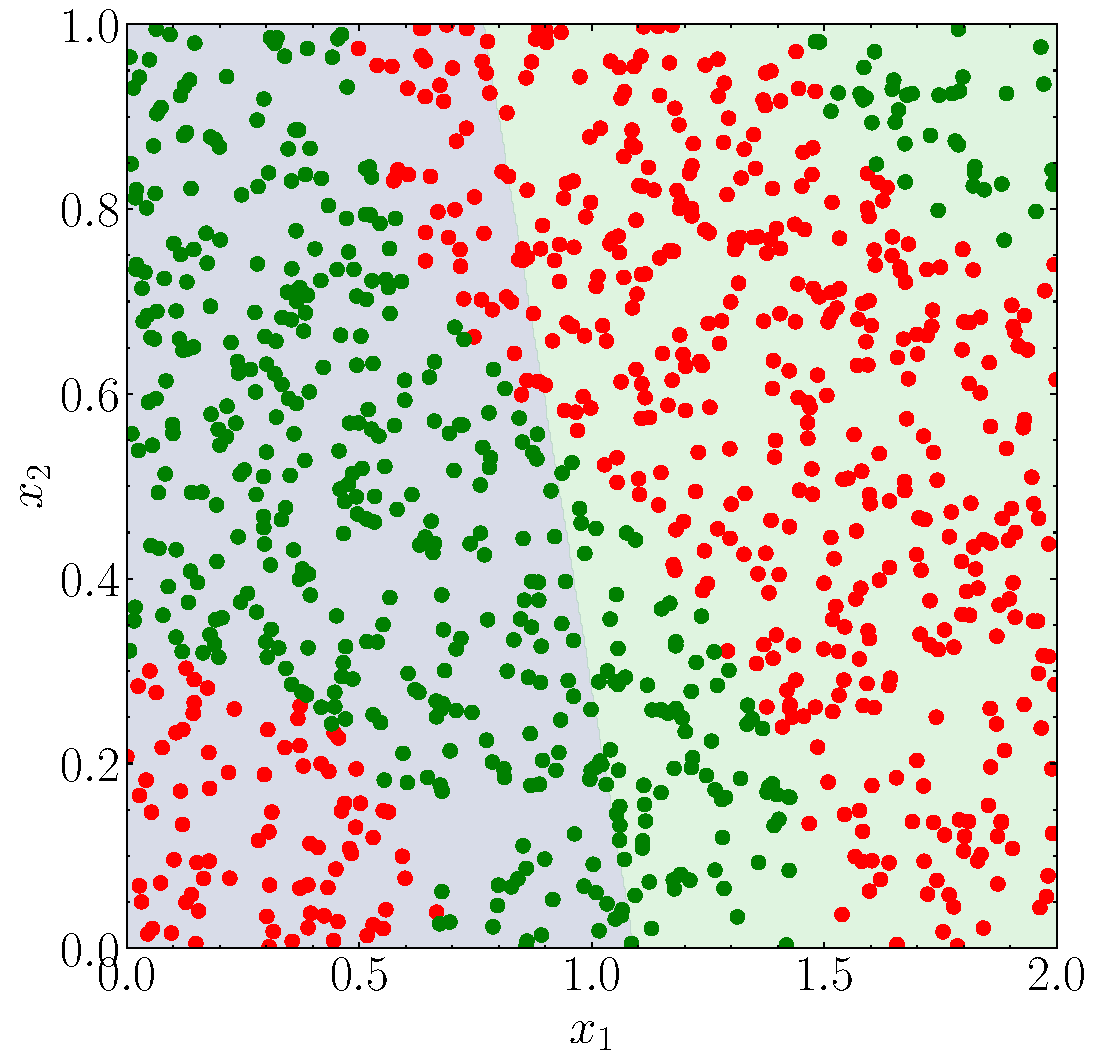
\includegraphics[width=1.5in]{../results/ex1/samples_LOG_dataset_noise0_size_1000}}
\subfigure[LOG, Classifier]{\label{fig:a}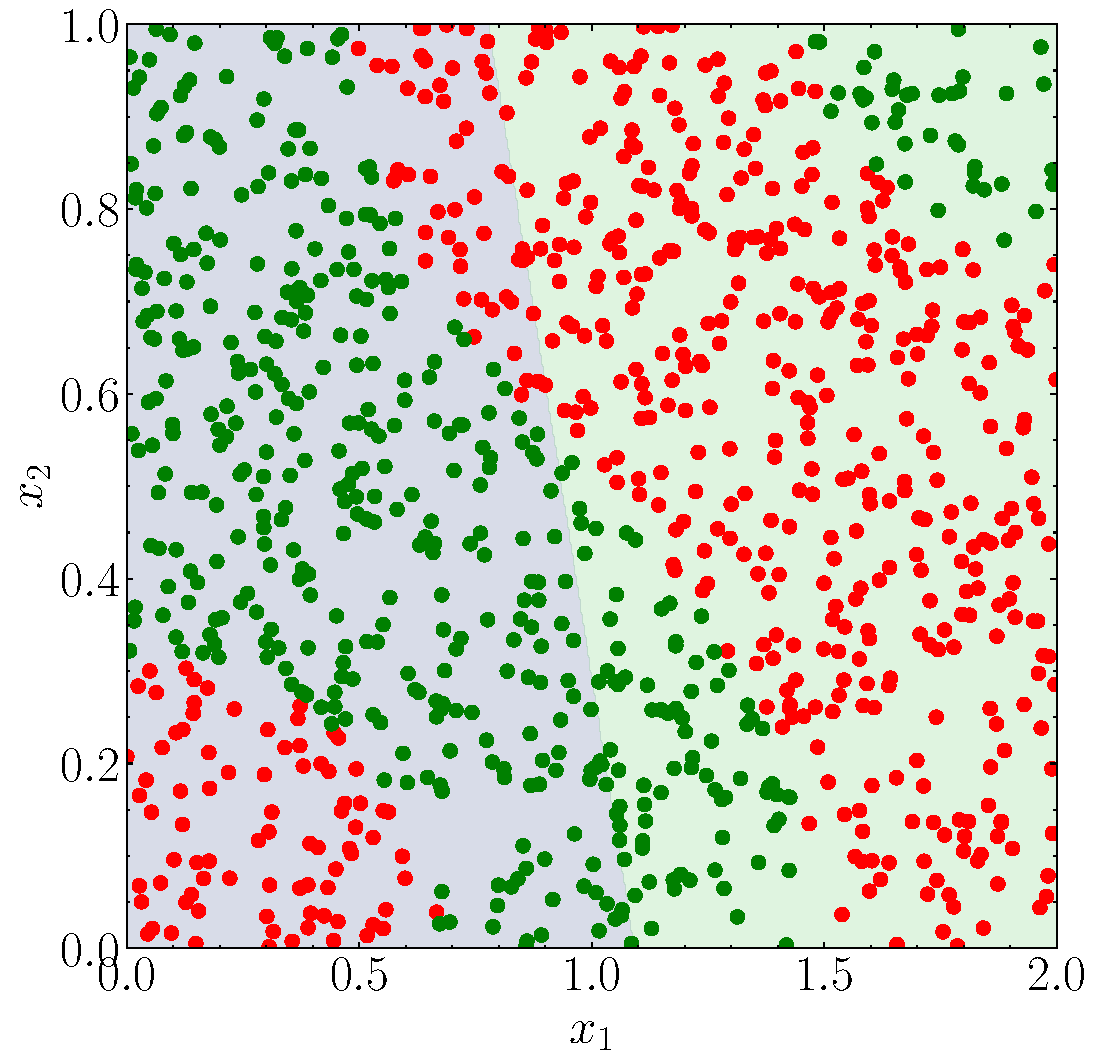
\includegraphics[width=1.5in]{../results/ex1/samples_LOG_dataset_noise0_size_1500}}
\subfigure[LOG, Classifier]{\label{fig:a}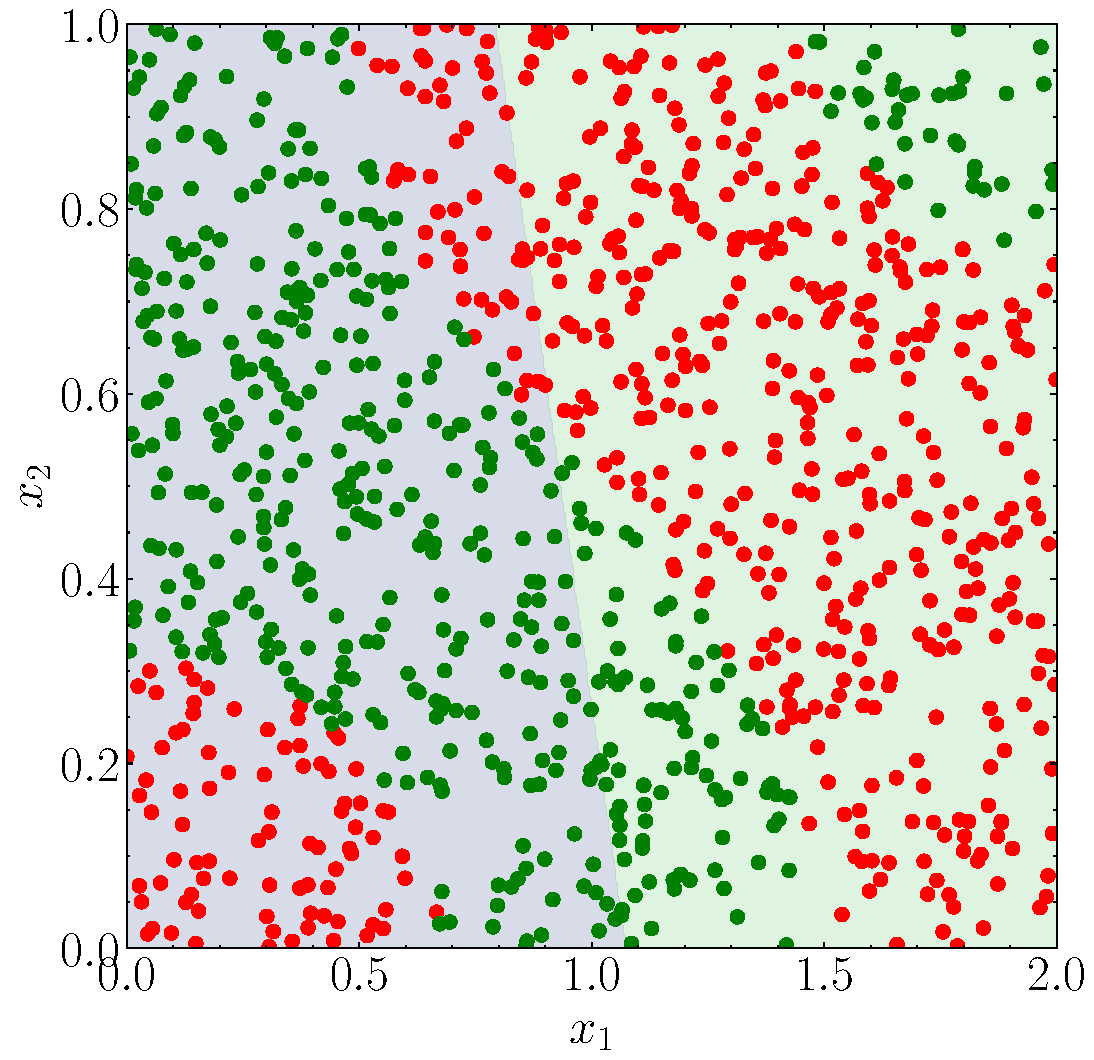
\includegraphics[width=1.5in]{../results/ex1/samples_LOG_dataset_noise0_size_2000}}

\caption{Logistic regression on 2D data with no label noise.}
\label{fig:LOG_ex1_noise0}
\end{figure}

{\it \bfseries Inferences:} It can be seen that the accuracy increases with increasing training size from $10$, $50$, $100$, $500$ and $999$ in both classifiers. Between the classifiers, logistic regression consistently gives better accuracy. Since the $x_{1}$ and $x_{2}$ coordinates are independent and Gamma distributed, it is known that the linear classifier has a slope of $-1$. It can be seen that logistic regression achieves this with fewer training samples. This is reflected in the accuracy. \\

\begin{figure}
\centering
\subfigure[Poly, Size $500$]{\label{fig:a}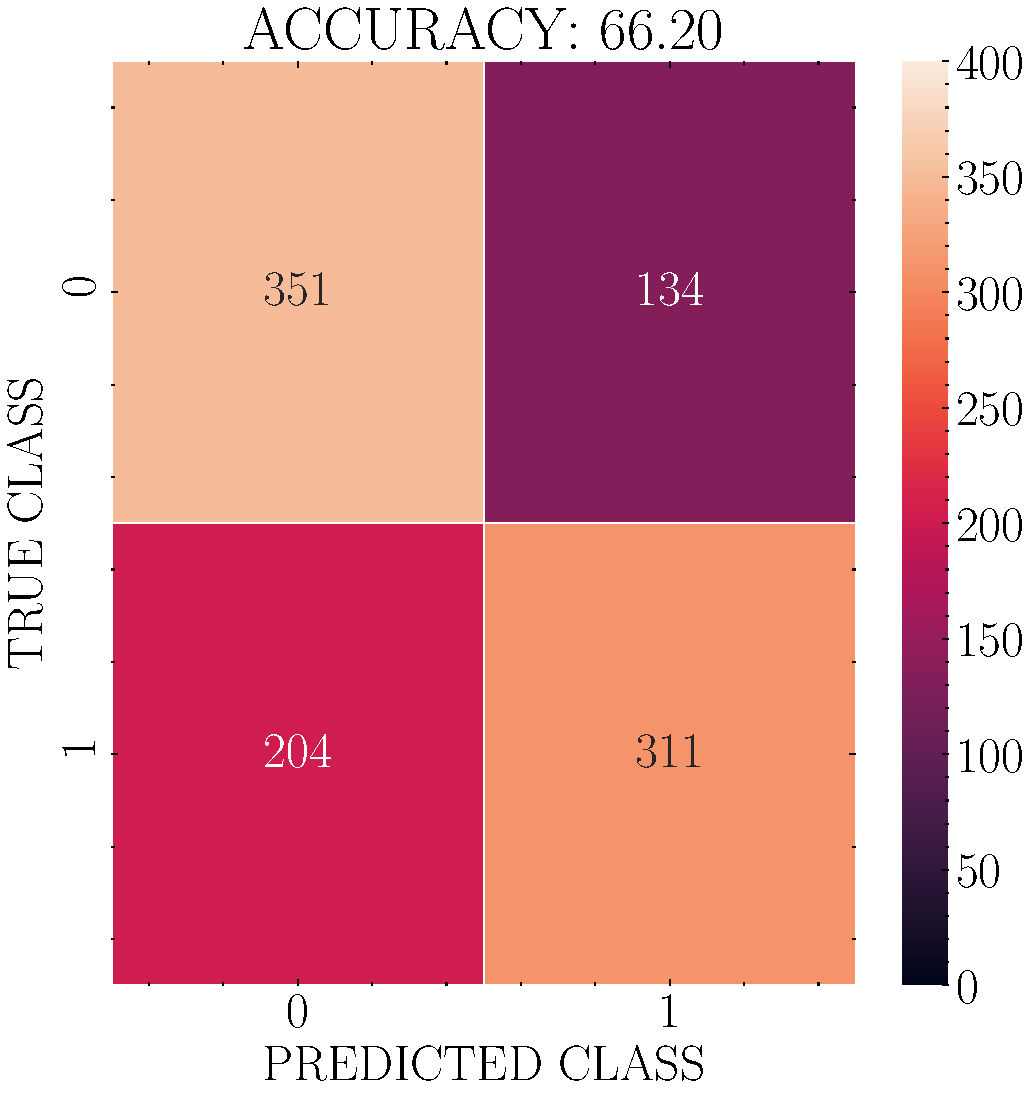
\includegraphics[width=1.5in]{../results/ex1/accuracy_SVM_dataset_noise20_method_poly_size_500}}
\subfigure[SVM-Poly, Classifier]{\label{fig:a}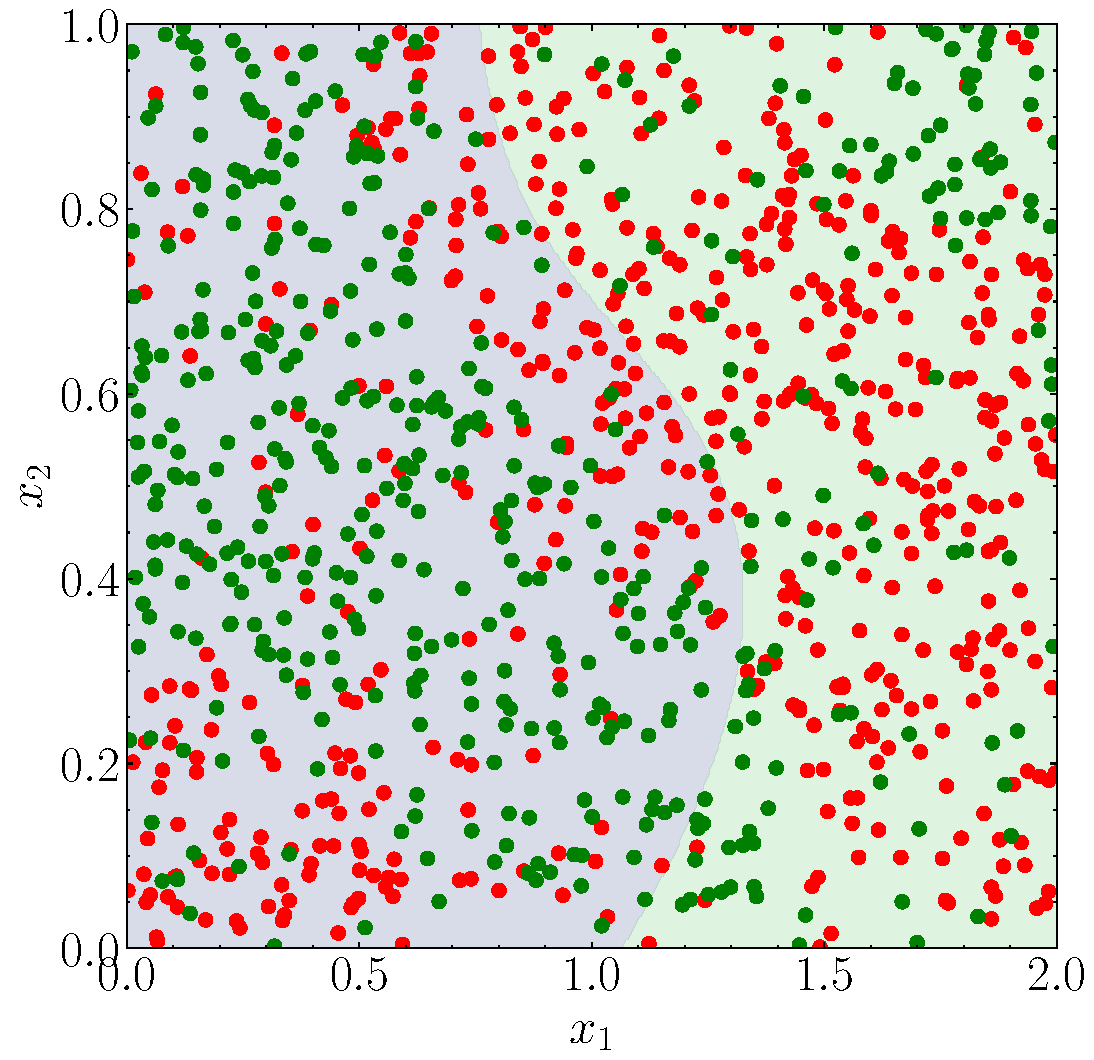
\includegraphics[width=1.5in]{../results/ex1/samples_SVM_dataset_noise20_method_poly_size_500}}
\subfigure[RBF, Size $500$]{\label{fig:a}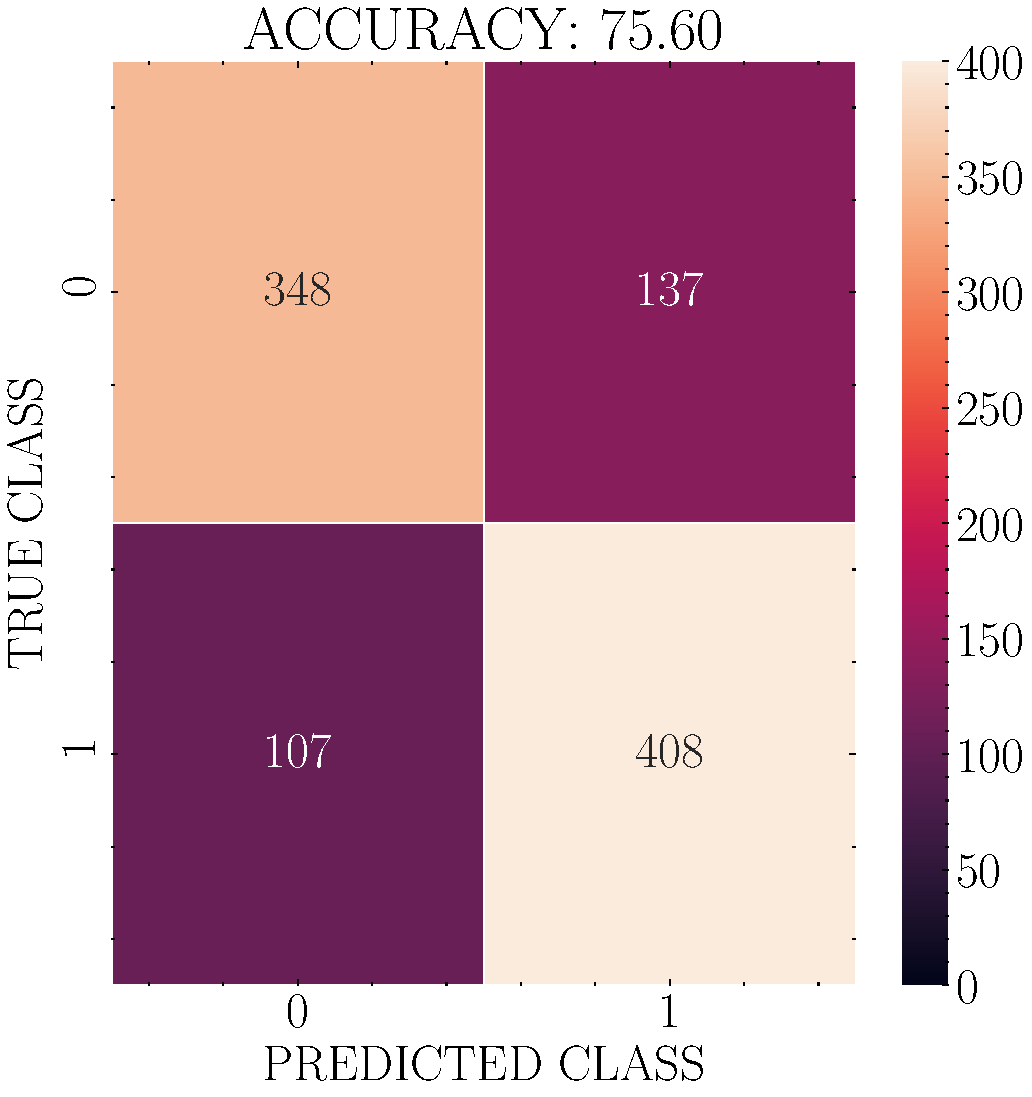
\includegraphics[width=1.5in]{../results/ex1/accuracy_SVM_dataset_noise20_method_rbf_size_500}}
\subfigure[SVM-RBF Classifier]{\label{fig:a}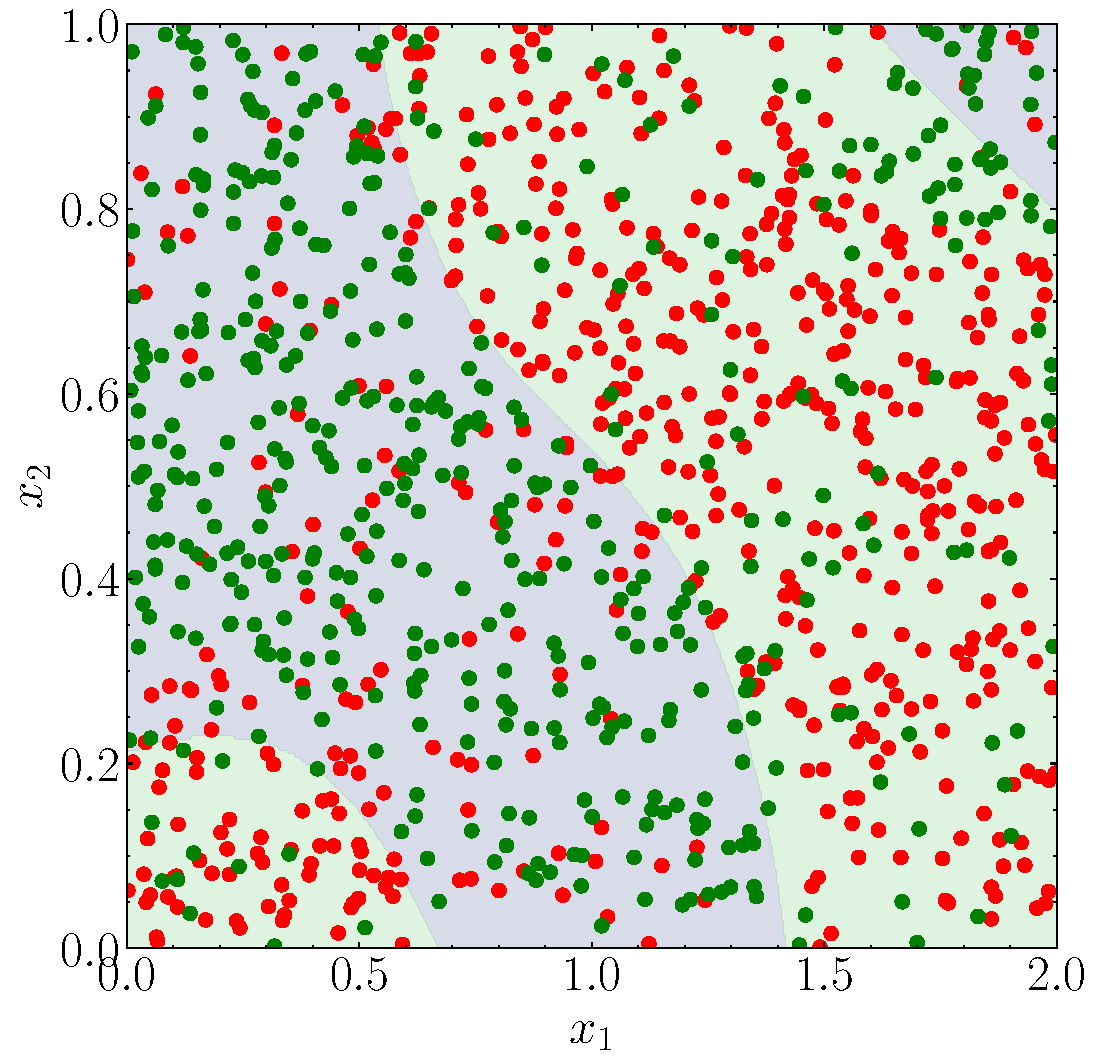
\includegraphics[width=1.5in]{../results/ex1/samples_SVM_dataset_noise20_method_rbf_size_500}}

\subfigure[Poly, Size $1000$]{\label{fig:a}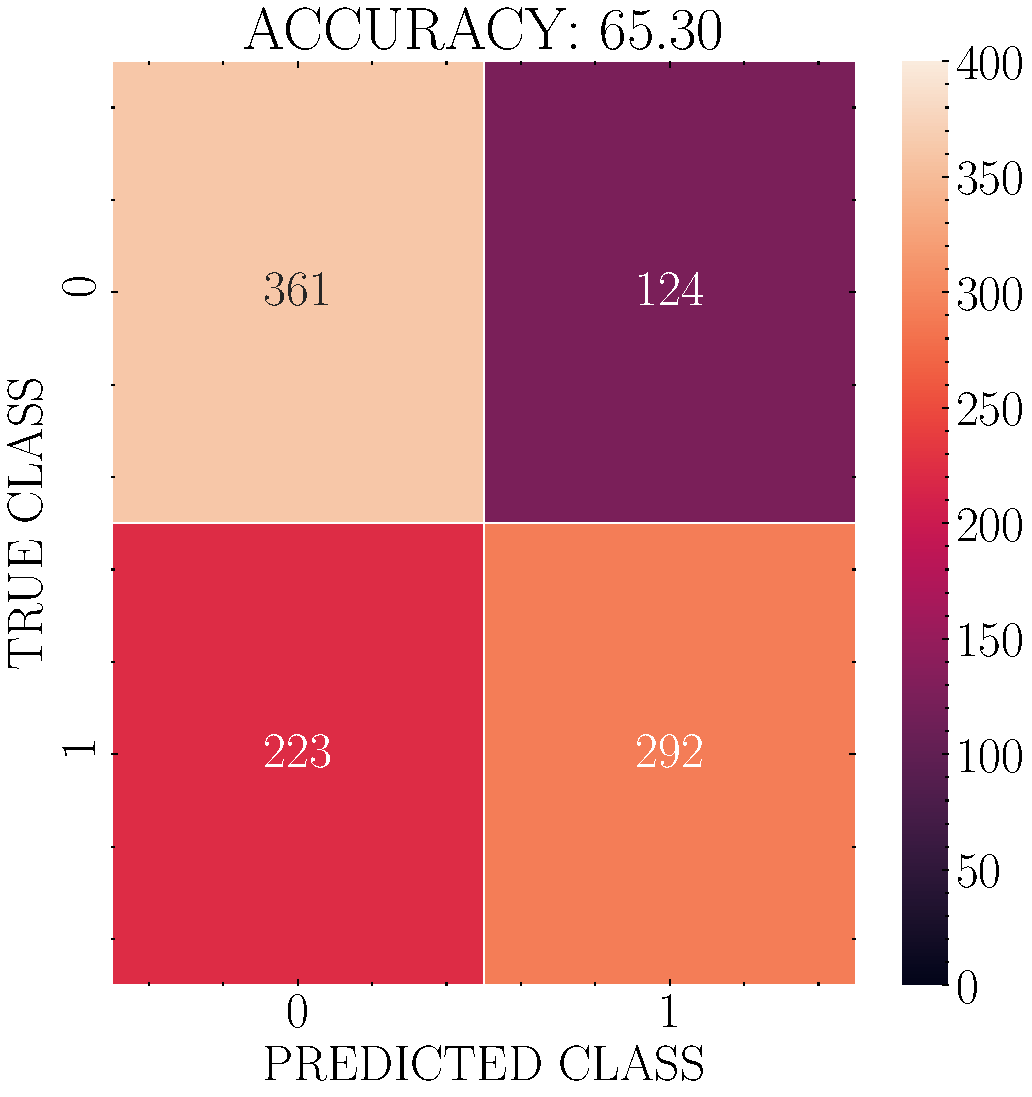
\includegraphics[width=1.5in]{../results/ex1/accuracy_SVM_dataset_noise20_method_poly_size_1000}}
\subfigure[SVM-Poly, Classifier]{\label{fig:a}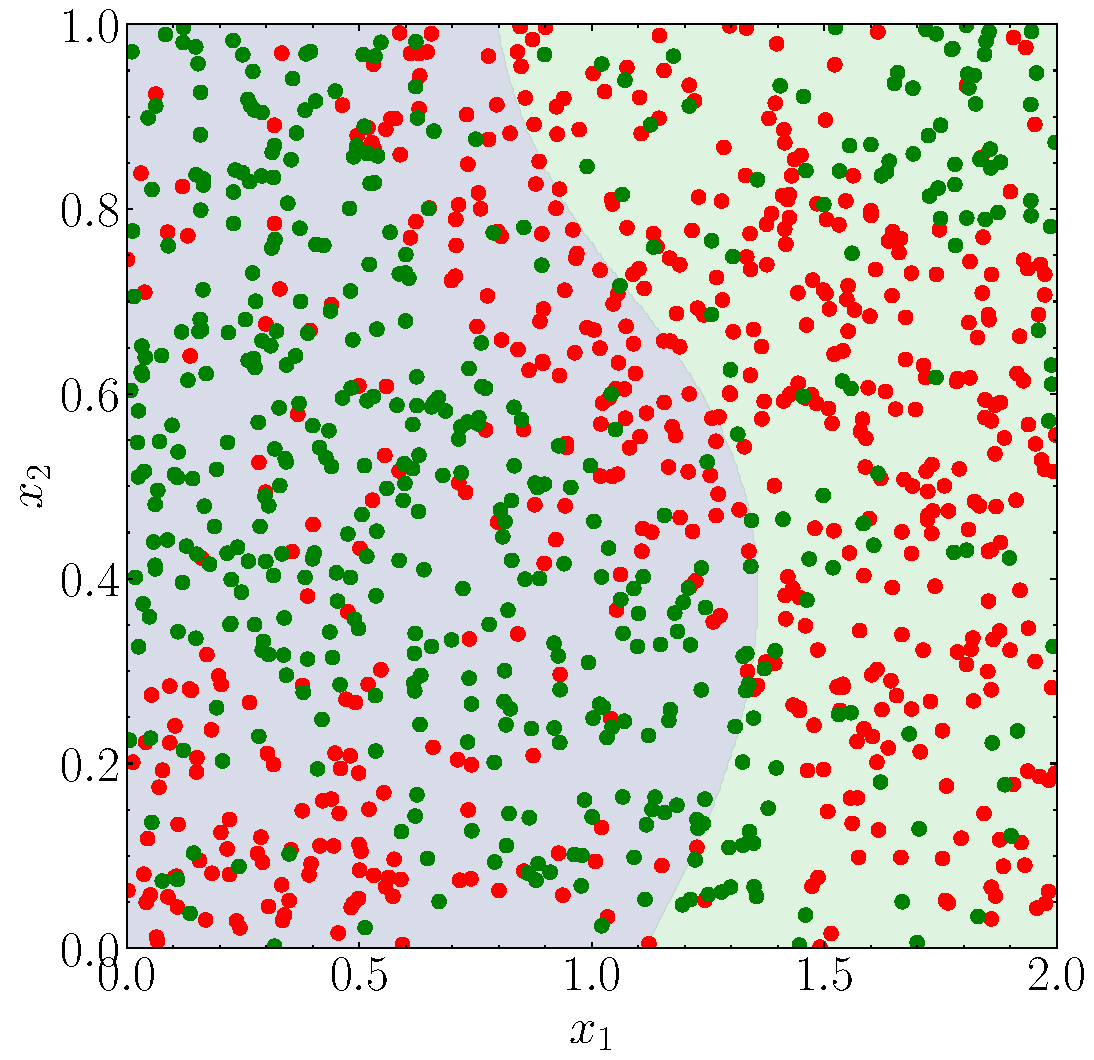
\includegraphics[width=1.5in]{../results/ex1/samples_SVM_dataset_noise20_method_poly_size_1000}}
\subfigure[RBF, Size $1000$]{\label{fig:a}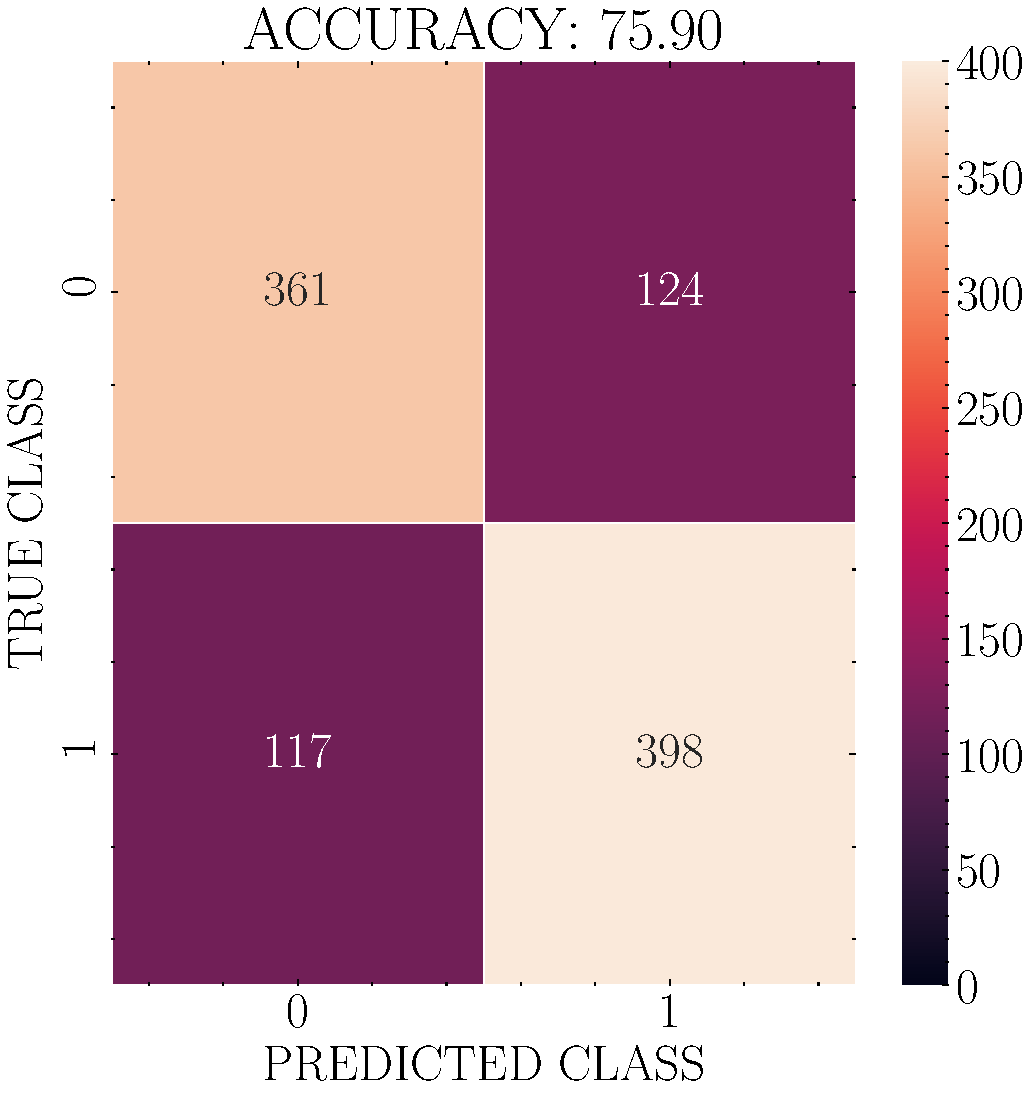
\includegraphics[width=1.5in]{../results/ex1/accuracy_SVM_dataset_noise20_method_rbf_size_1000}}
\subfigure[SVM-RBF Classifier]{\label{fig:a}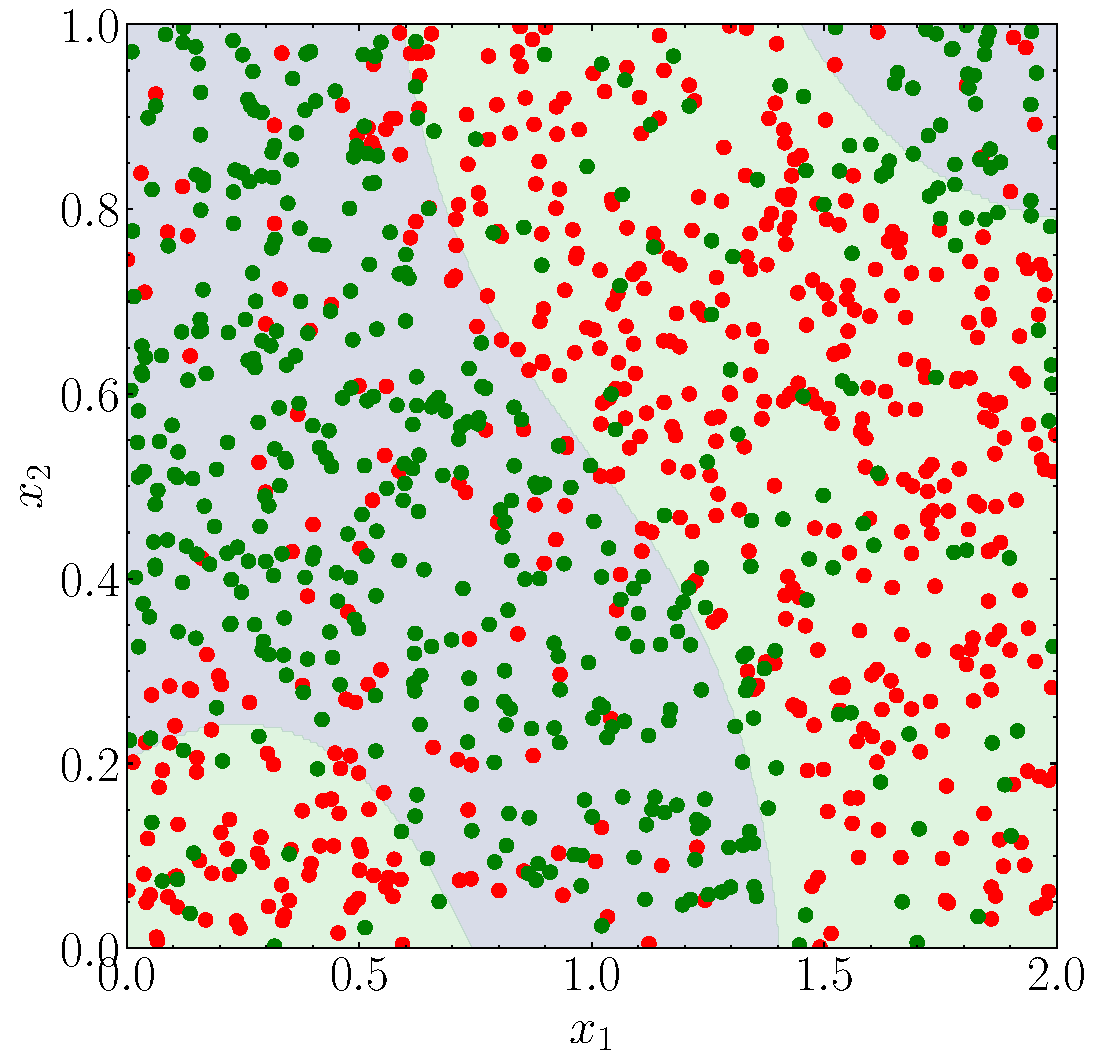
\includegraphics[width=1.5in]{../results/ex1/samples_SVM_dataset_noise20_method_rbf_size_1000}}

\subfigure[Poly, Size $1500$]{\label{fig:a}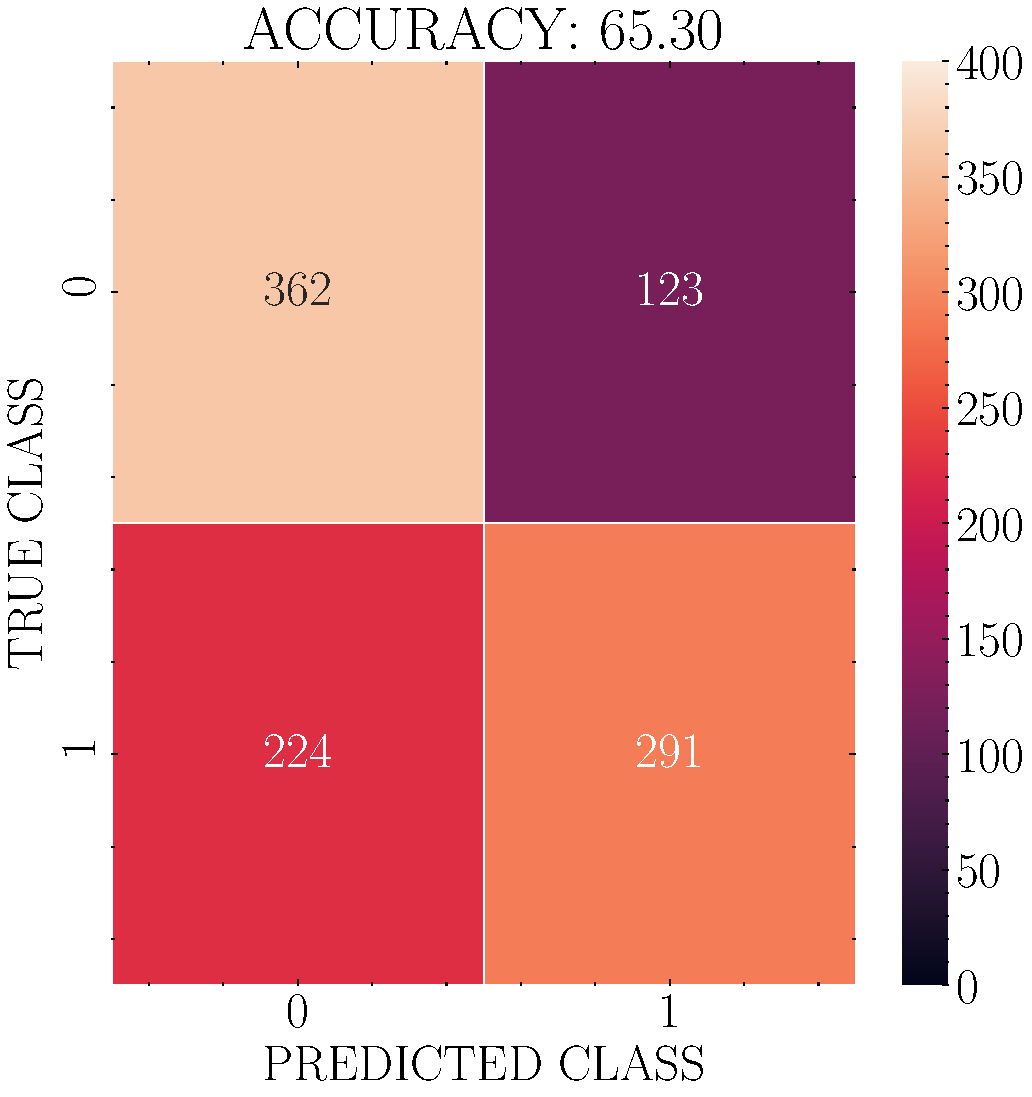
\includegraphics[width=1.5in]{../results/ex1/accuracy_SVM_dataset_noise20_method_poly_size_1500}}
\subfigure[SVM-Poly, Classifier]{\label{fig:a}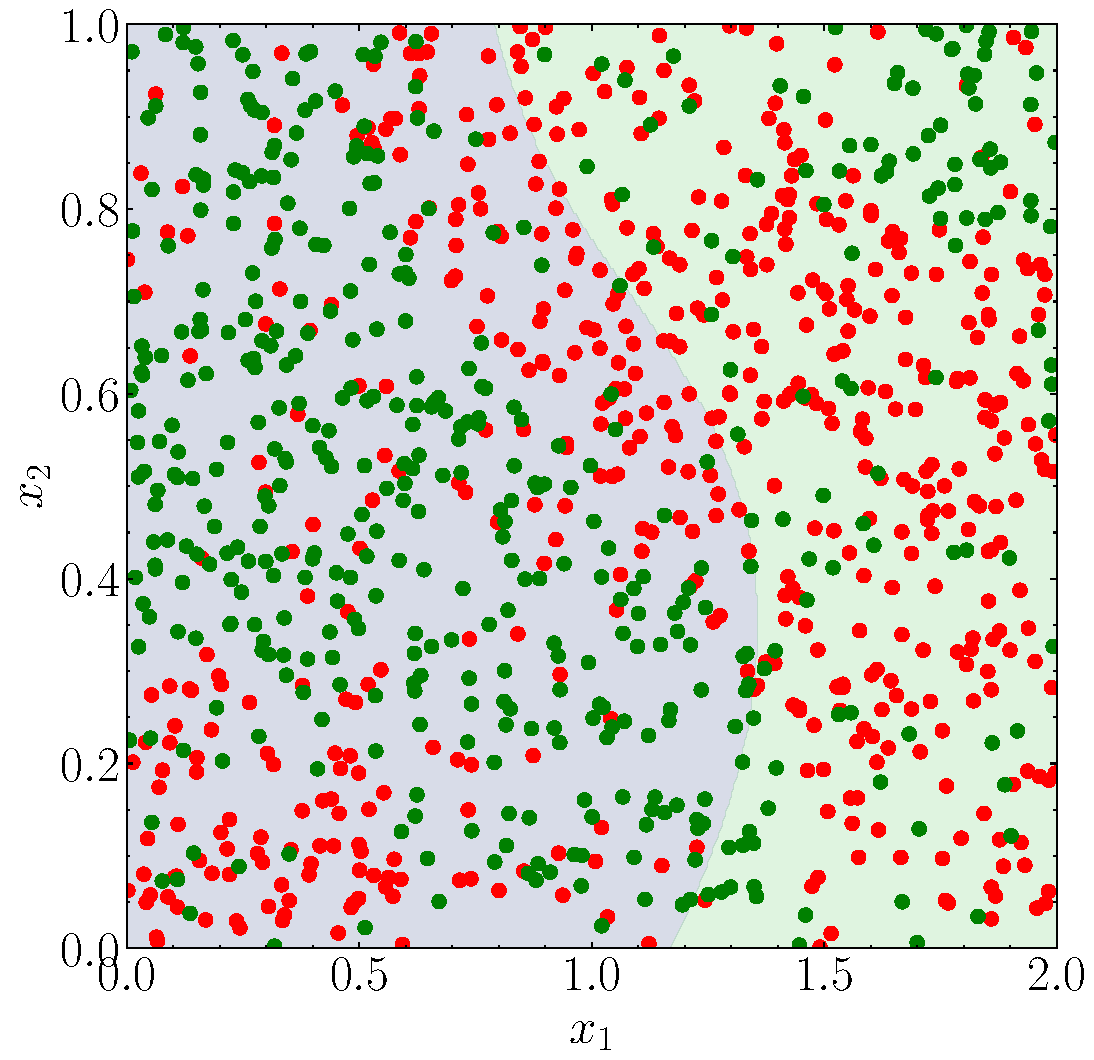
\includegraphics[width=1.5in]{../results/ex1/samples_SVM_dataset_noise20_method_poly_size_1500}}
\subfigure[RBF, Size $1500$]{\label{fig:a}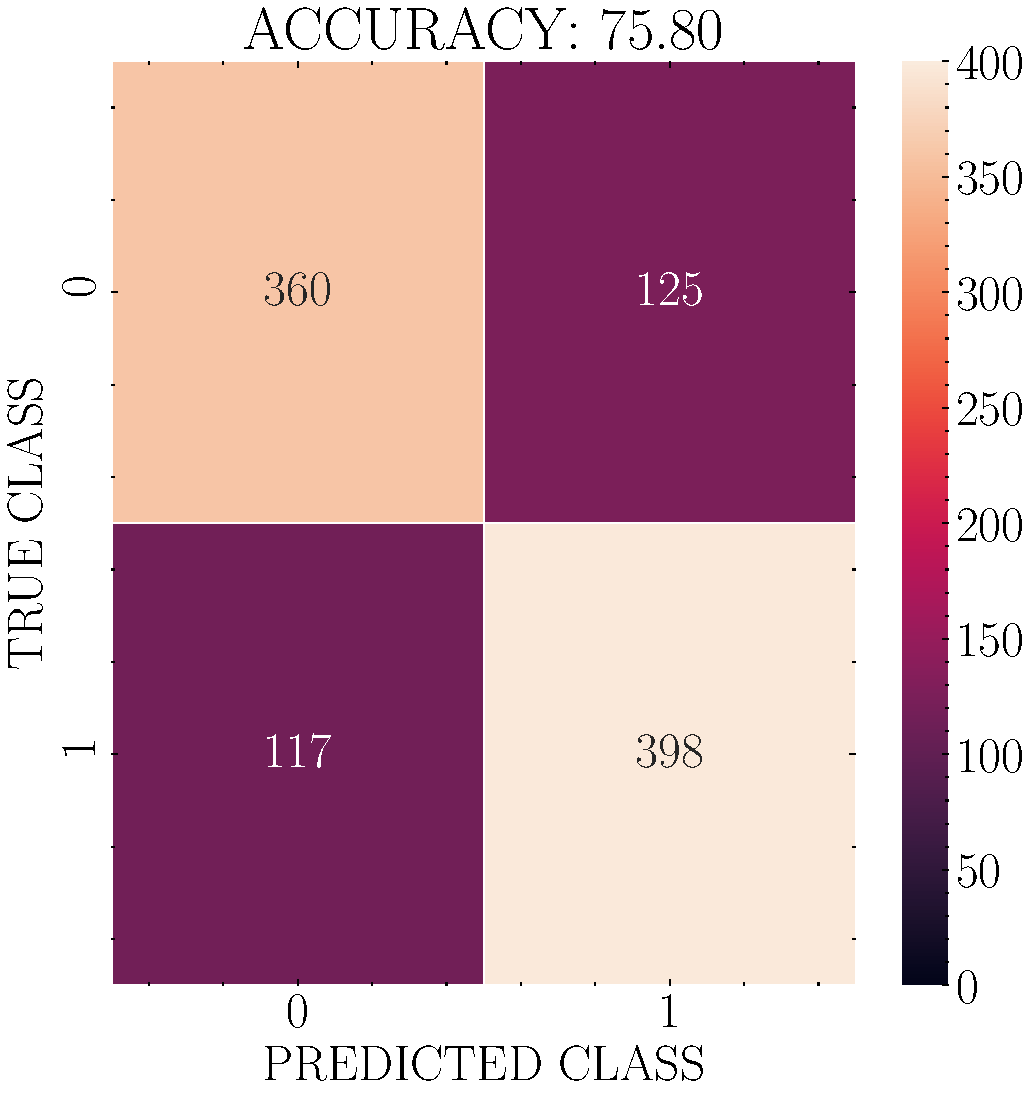
\includegraphics[width=1.5in]{../results/ex1/accuracy_SVM_dataset_noise20_method_rbf_size_1500}}
\subfigure[SVM-RBF Classifier]{\label{fig:a}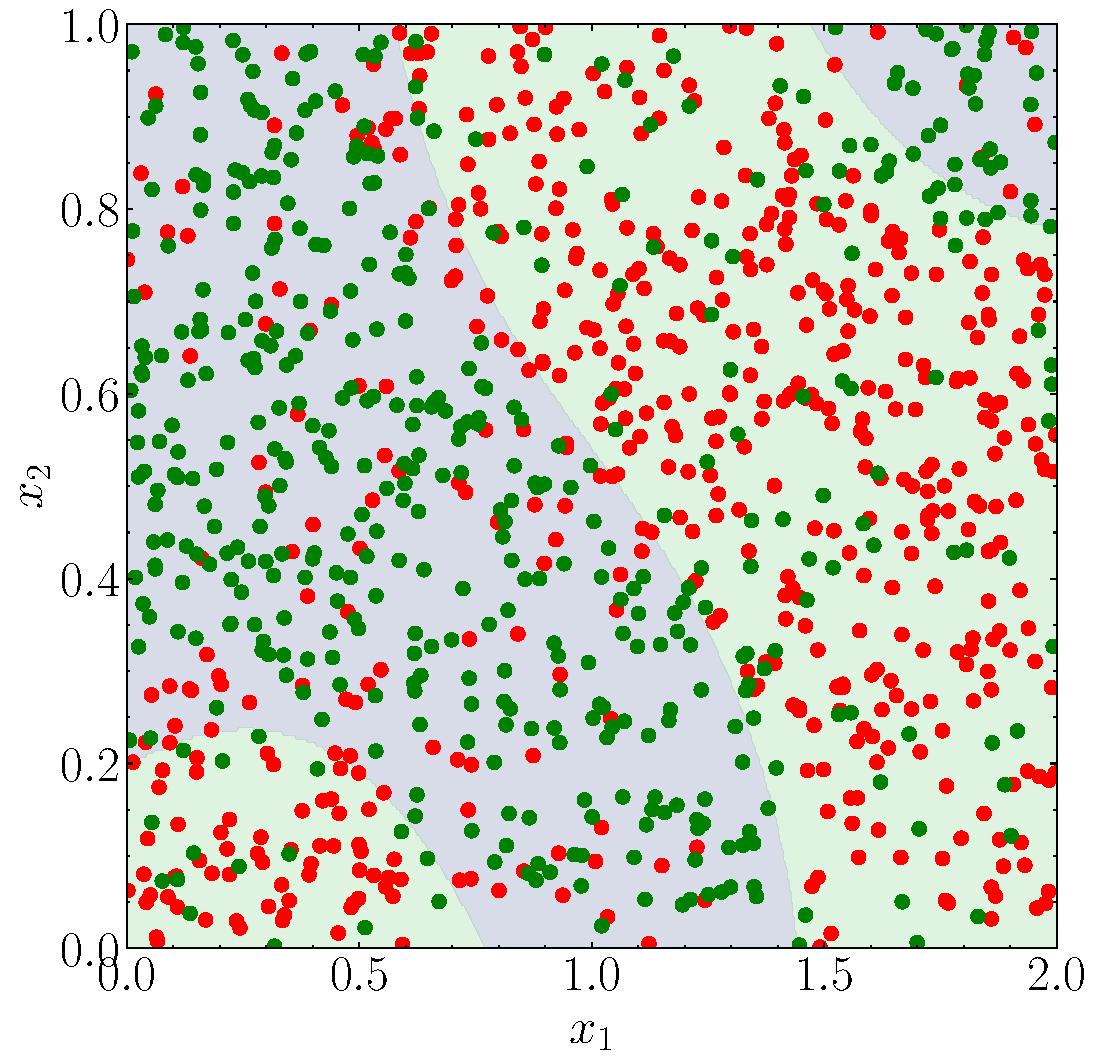
\includegraphics[width=1.5in]{../results/ex1/samples_SVM_dataset_noise20_method_rbf_size_1500}}

\subfigure[Poly, Size $2000$]{\label{fig:a}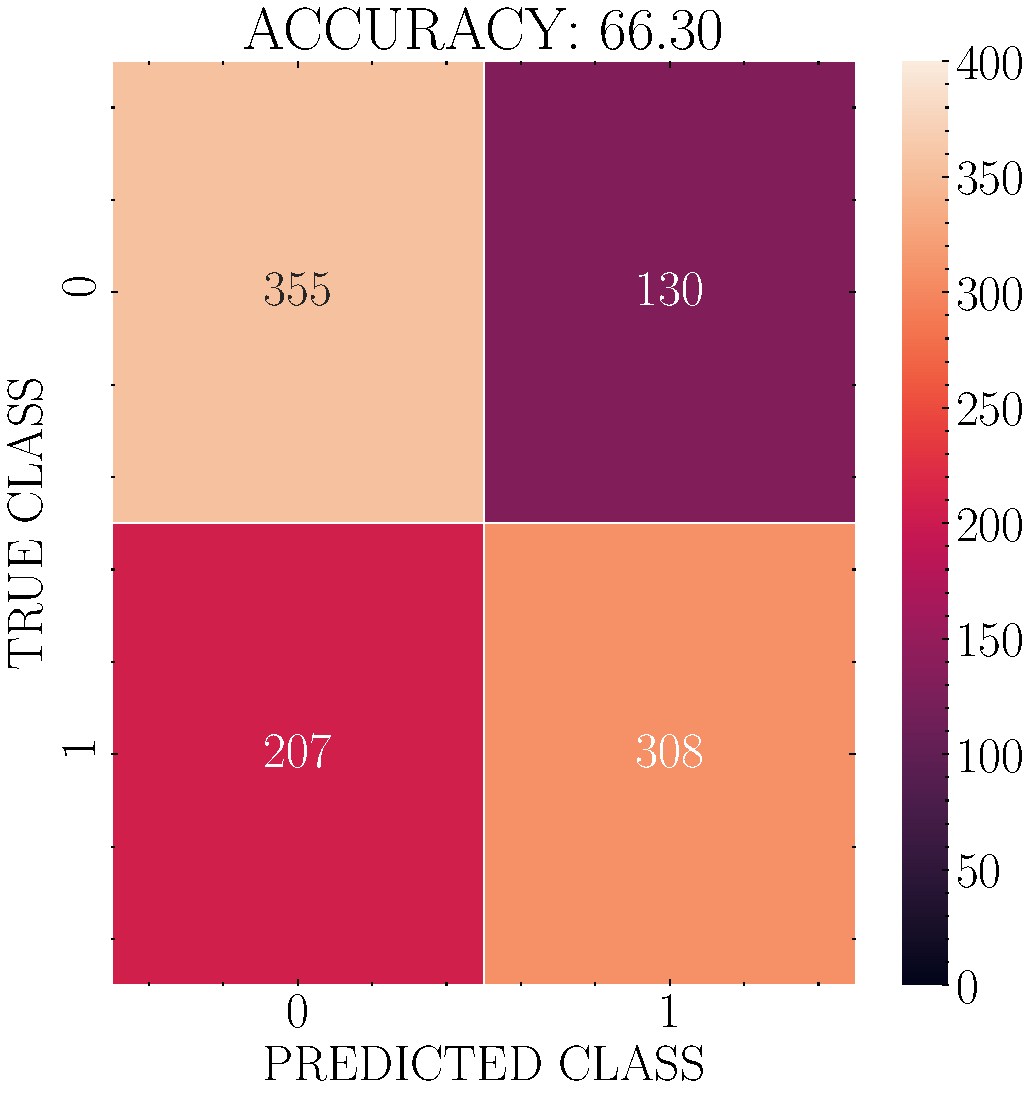
\includegraphics[width=1.5in]{../results/ex1/accuracy_SVM_dataset_noise20_method_poly_size_2000}}
\subfigure[SVM-Poly, Classifier]{\label{fig:a}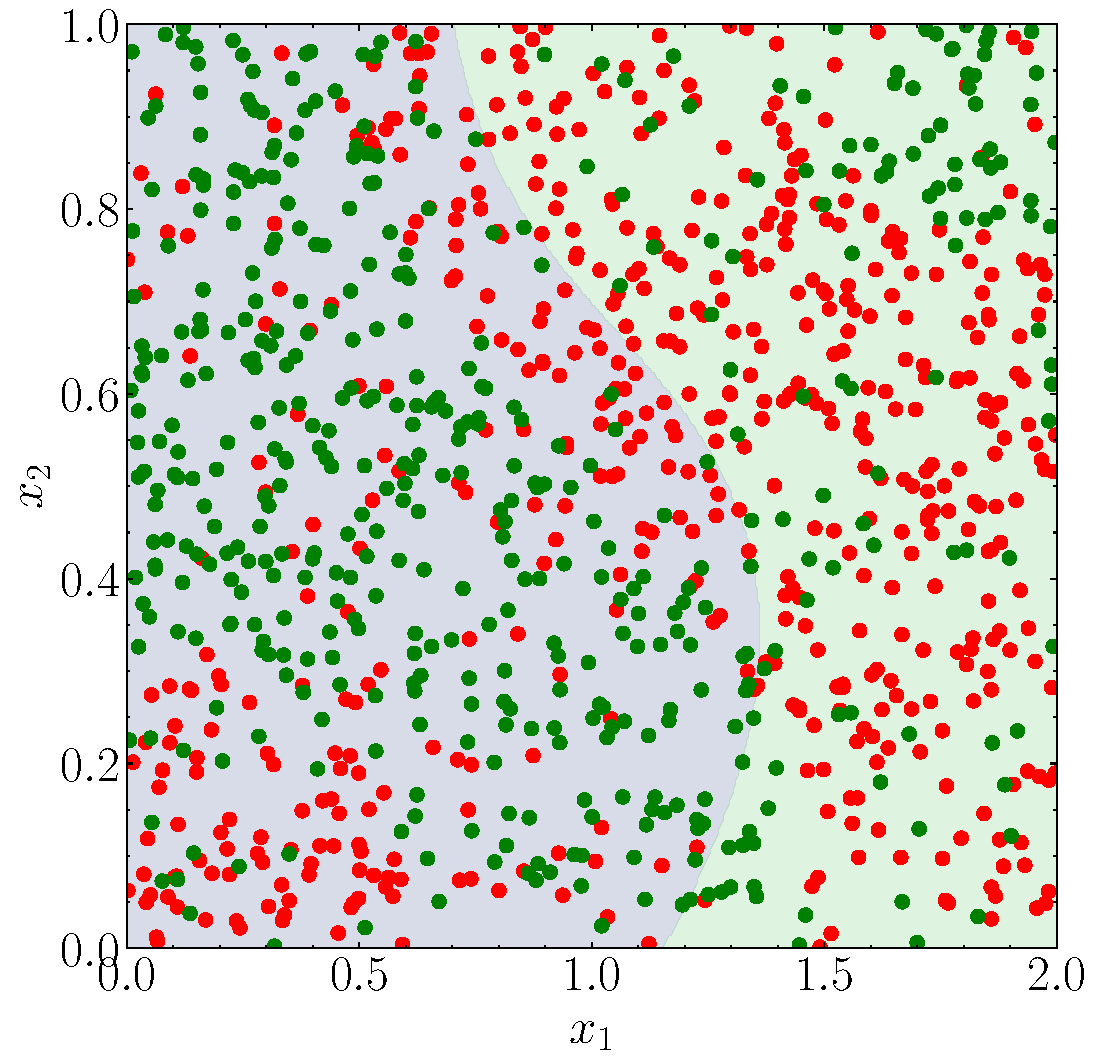
\includegraphics[width=1.5in]{../results/ex1/samples_SVM_dataset_noise20_method_poly_size_2000}}
\subfigure[RBF, Size $2000$]{\label{fig:a}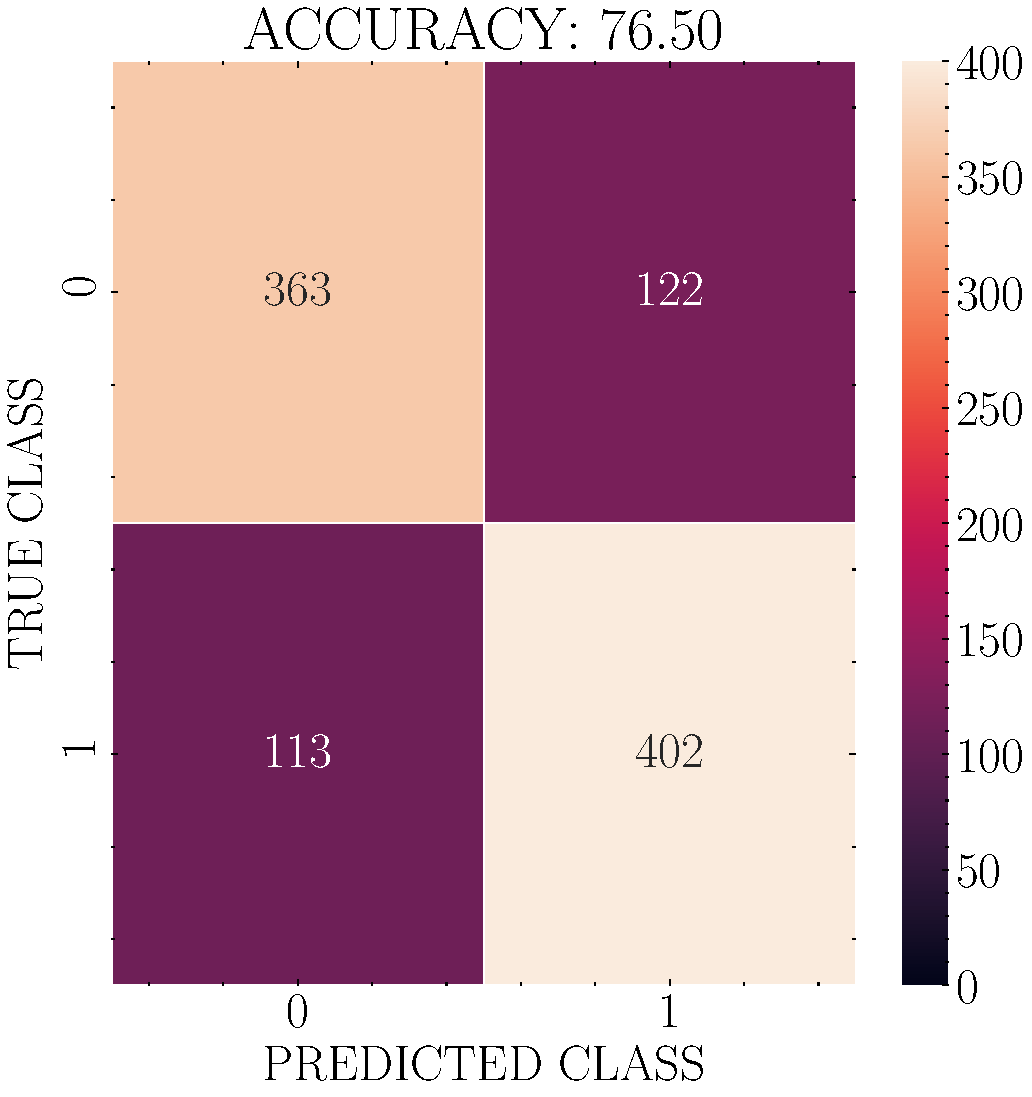
\includegraphics[width=1.5in]{../results/ex1/accuracy_SVM_dataset_noise20_method_rbf_size_2000}}
\subfigure[SVM-RBF Classifier]{\label{fig:a}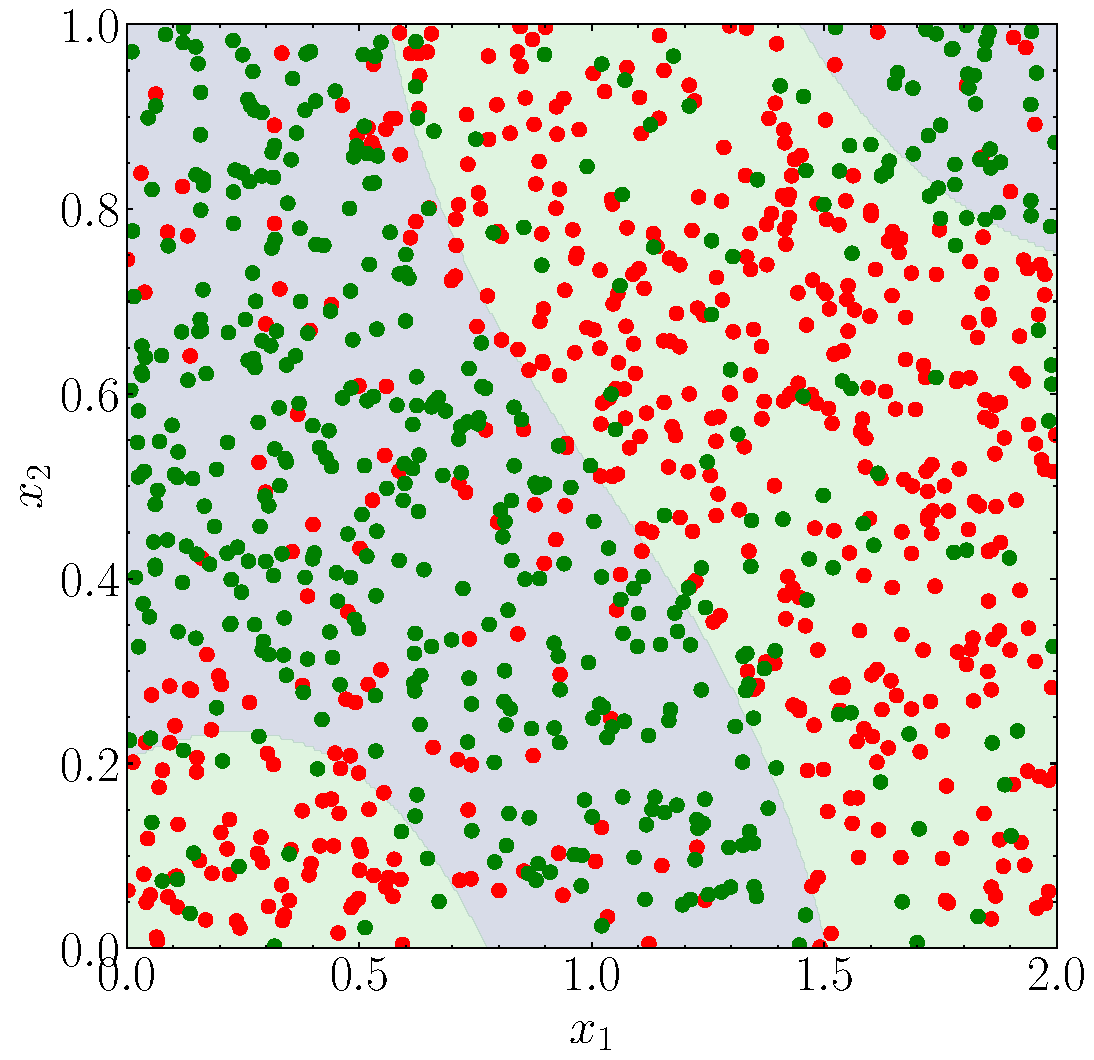
\includegraphics[width=1.5in]{../results/ex1/samples_SVM_dataset_noise20_method_rbf_size_2000}}

\caption{Support vector machines with polynomial kernel of degree $3$ and Gaussian kernel on 2D data with $20\%$ label noise.}
\label{fig:SVM_ex1_noise20}
\end{figure}

\begin{figure}
\centering
\subfigure[Poly, Size $500$]{\label{fig:a}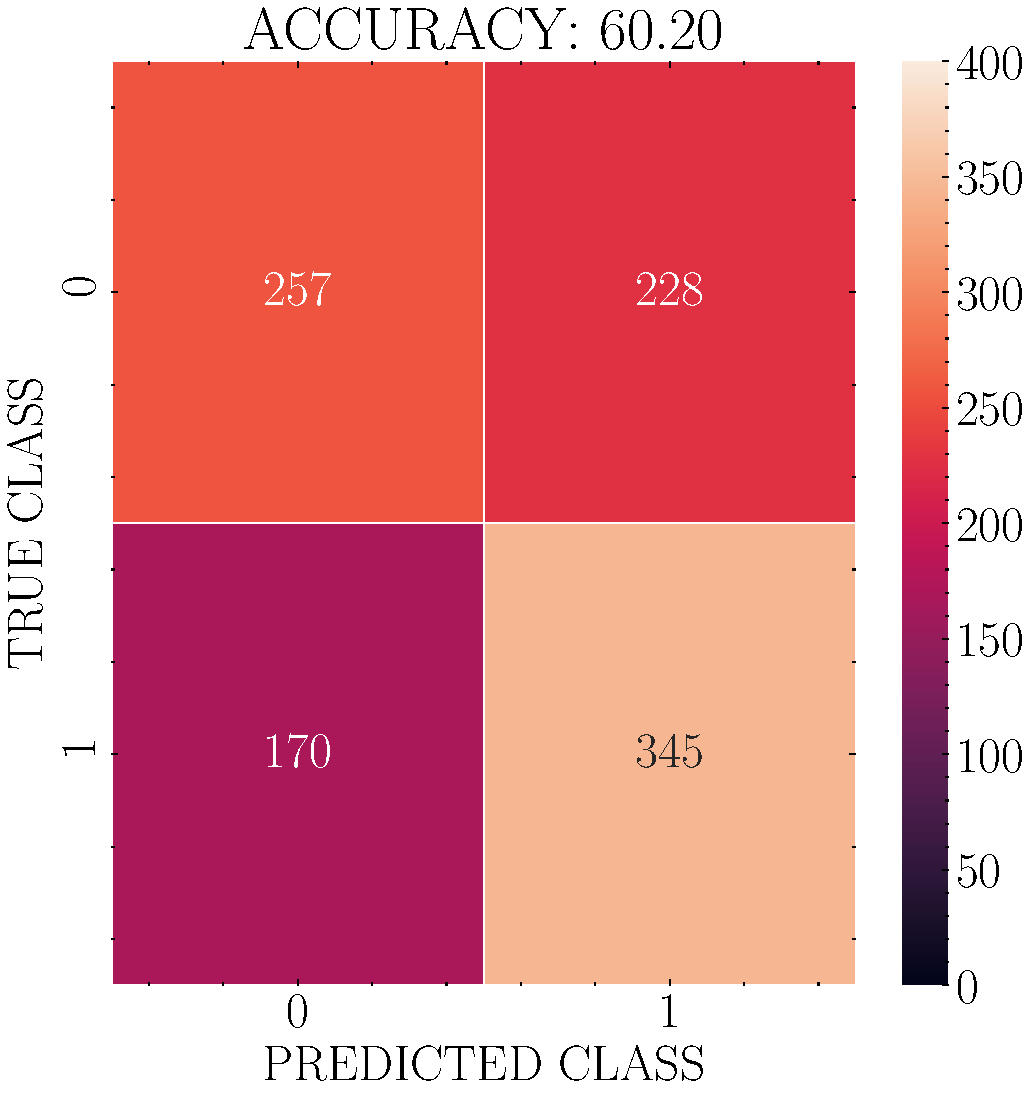
\includegraphics[width=1.5in]{../results/ex1/accuracy_LOG_dataset_noise20_size_500}}
\subfigure[Poly, Size $1000$]{\label{fig:a}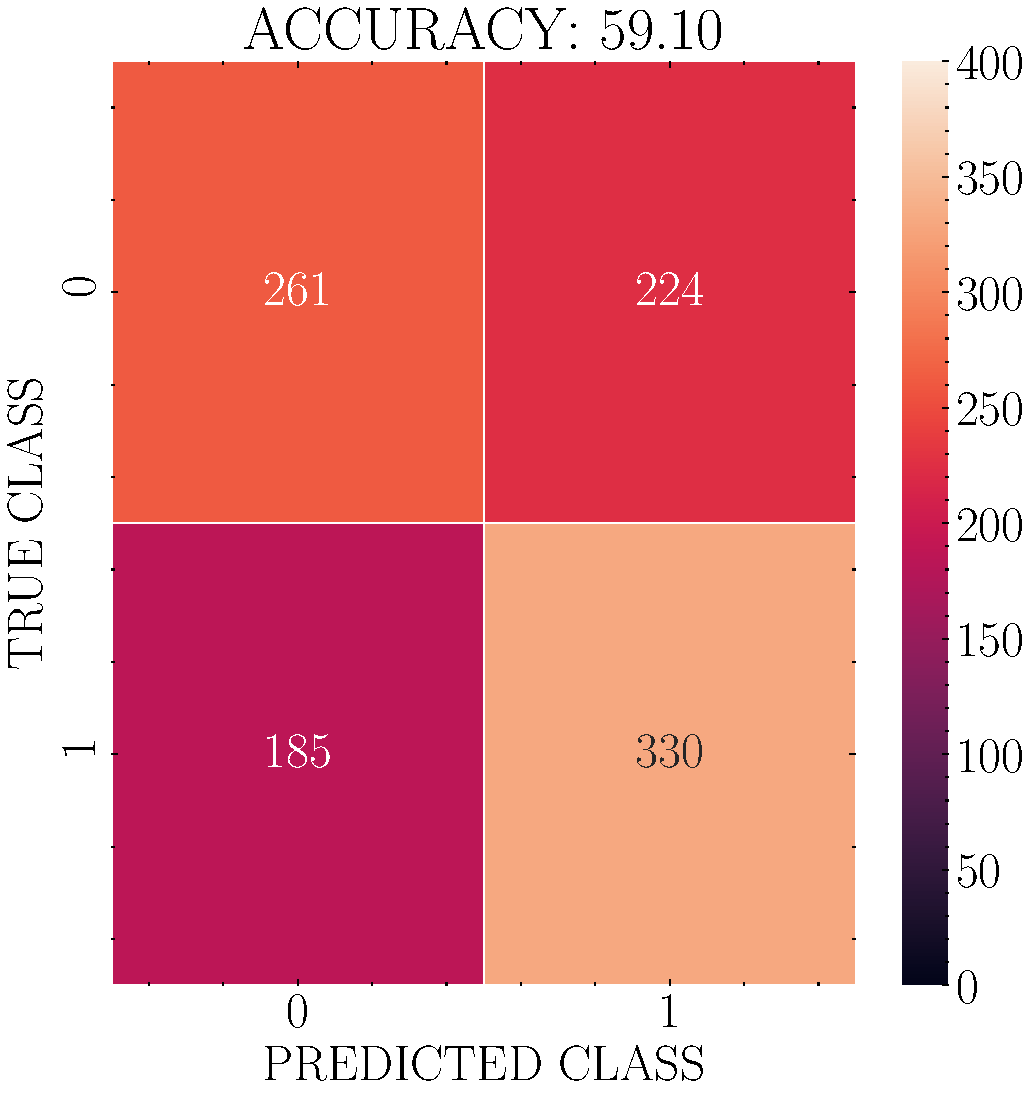
\includegraphics[width=1.5in]{../results/ex1/accuracy_LOG_dataset_noise20_size_1000}}
\subfigure[Poly, Size $1500$]{\label{fig:a}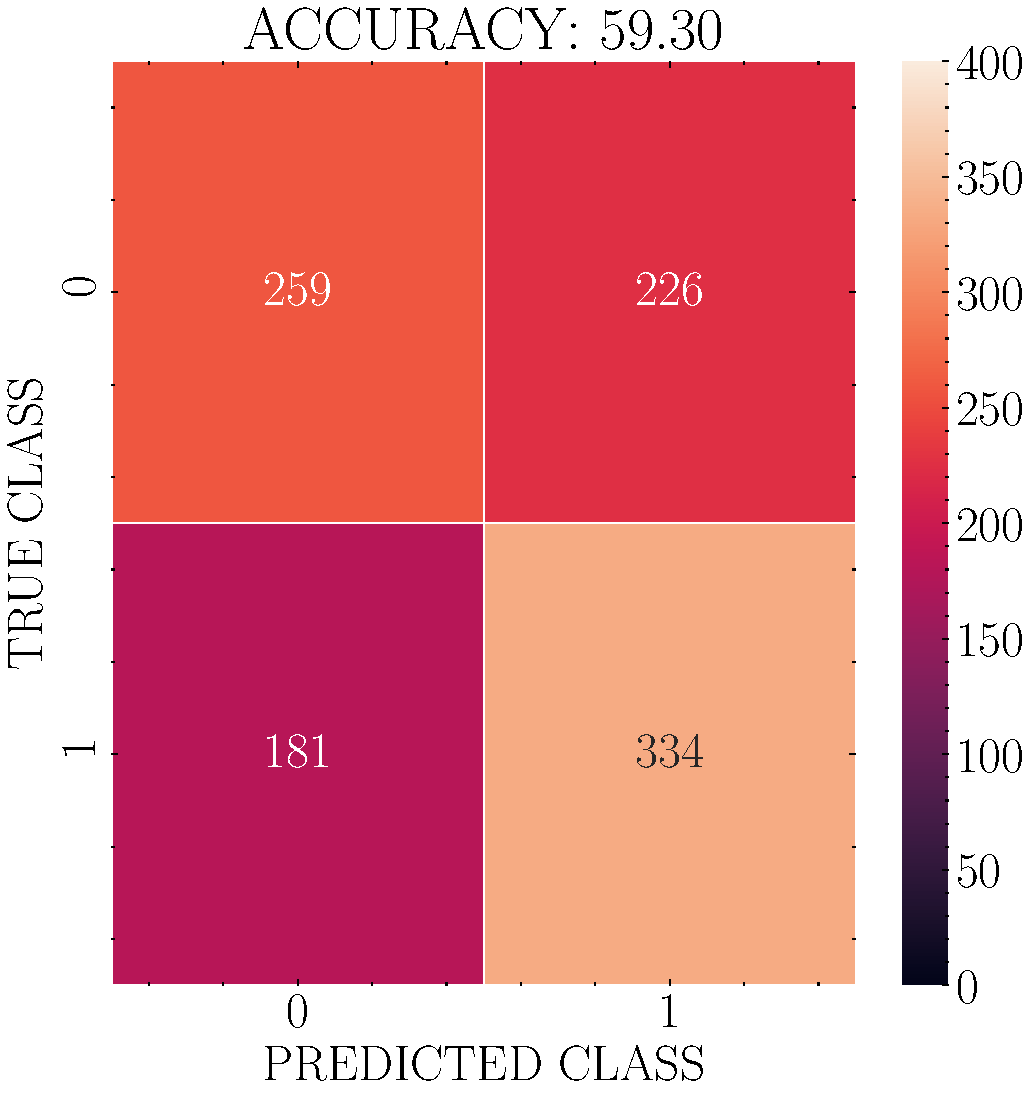
\includegraphics[width=1.5in]{../results/ex1/accuracy_LOG_dataset_noise20_size_1500}}
\subfigure[Poly, Size $2000$]{\label{fig:a}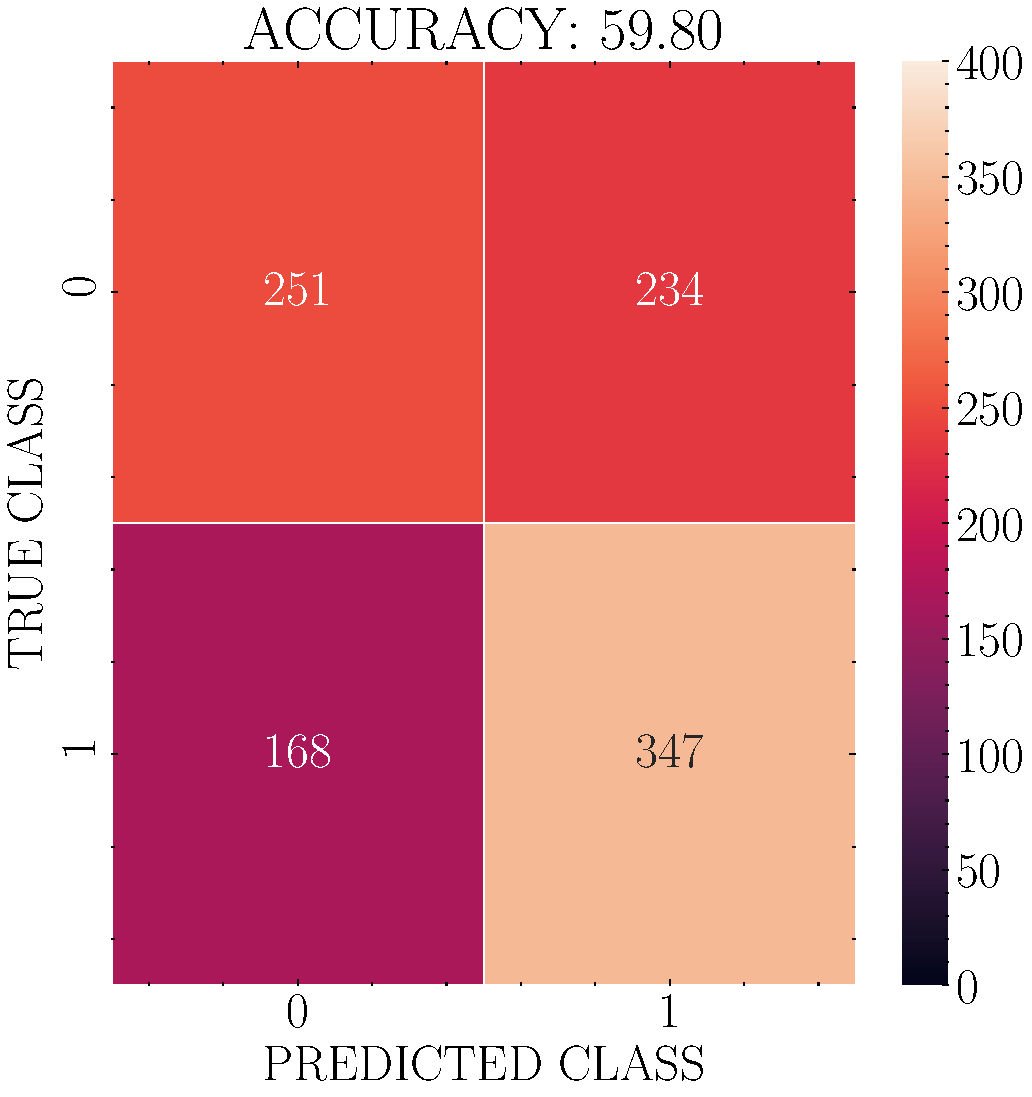
\includegraphics[width=1.5in]{../results/ex1/accuracy_LOG_dataset_noise20_size_2000}}

\subfigure[LOG, Classifier]{\label{fig:a}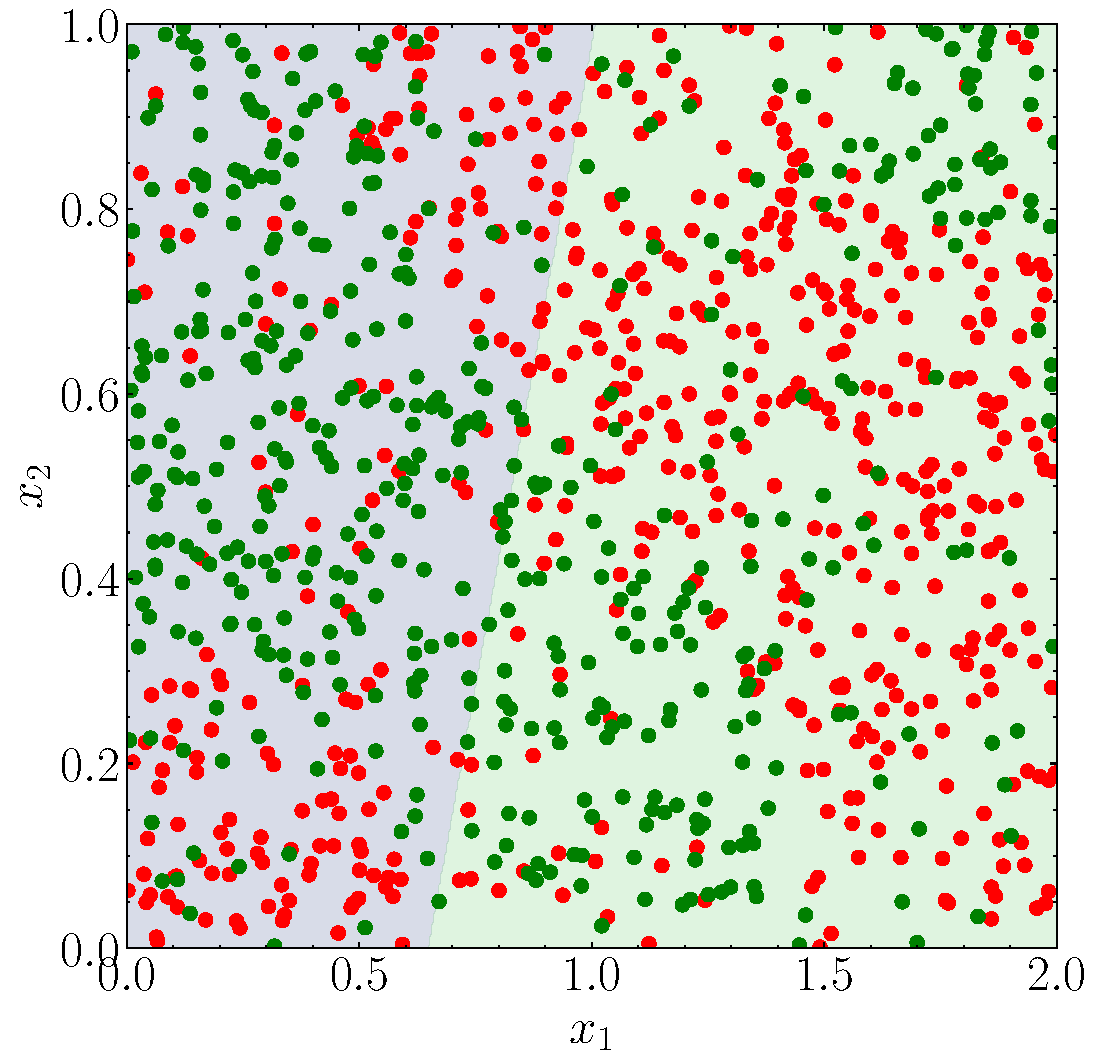
\includegraphics[width=1.5in]{../results/ex1/samples_LOG_dataset_noise20_size_500}}
\subfigure[LOG, Classifier]{\label{fig:a}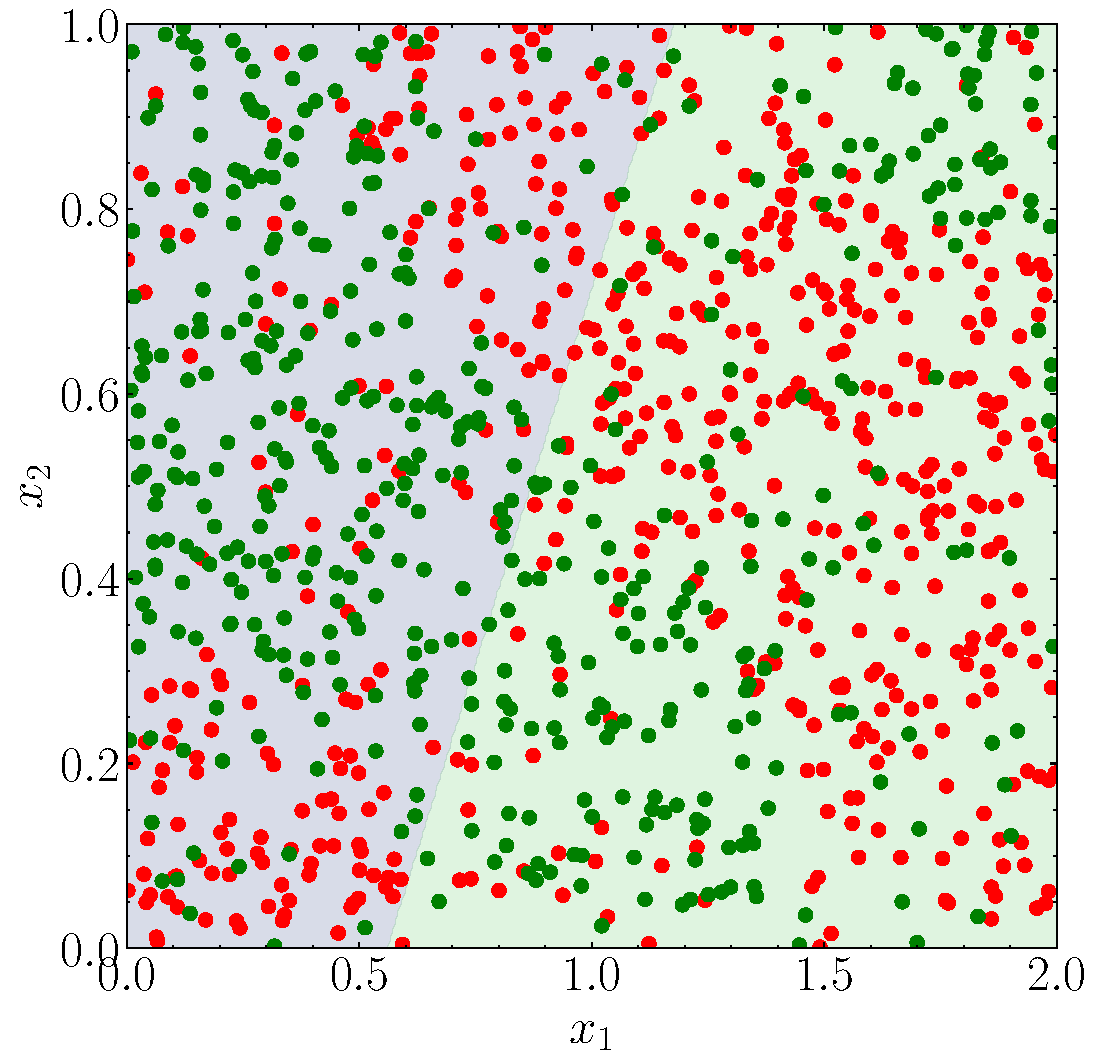
\includegraphics[width=1.5in]{../results/ex1/samples_LOG_dataset_noise20_size_1000}}
\subfigure[LOG, Classifier]{\label{fig:a}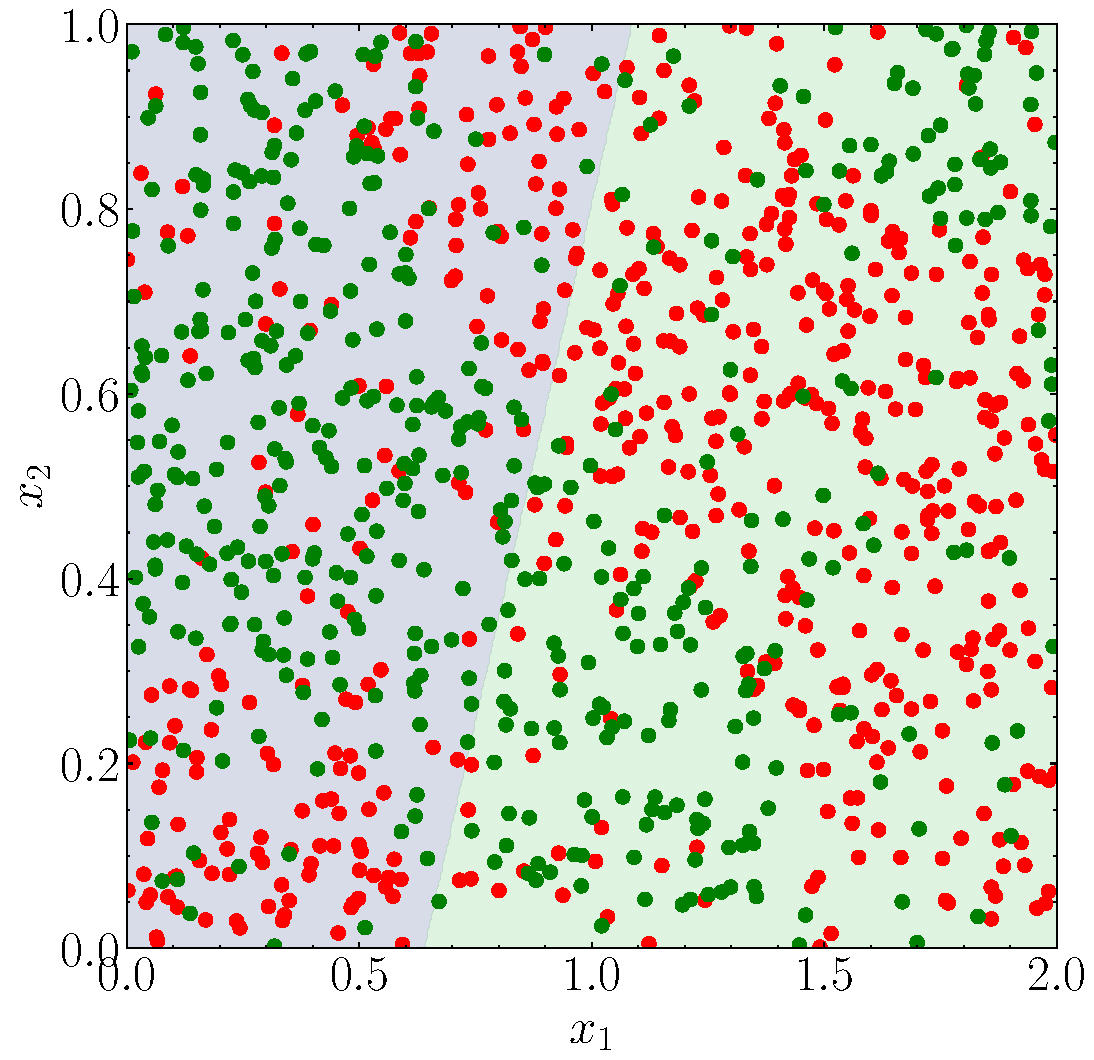
\includegraphics[width=1.5in]{../results/ex1/samples_LOG_dataset_noise20_size_1500}}
\subfigure[LOG, Classifier]{\label{fig:a}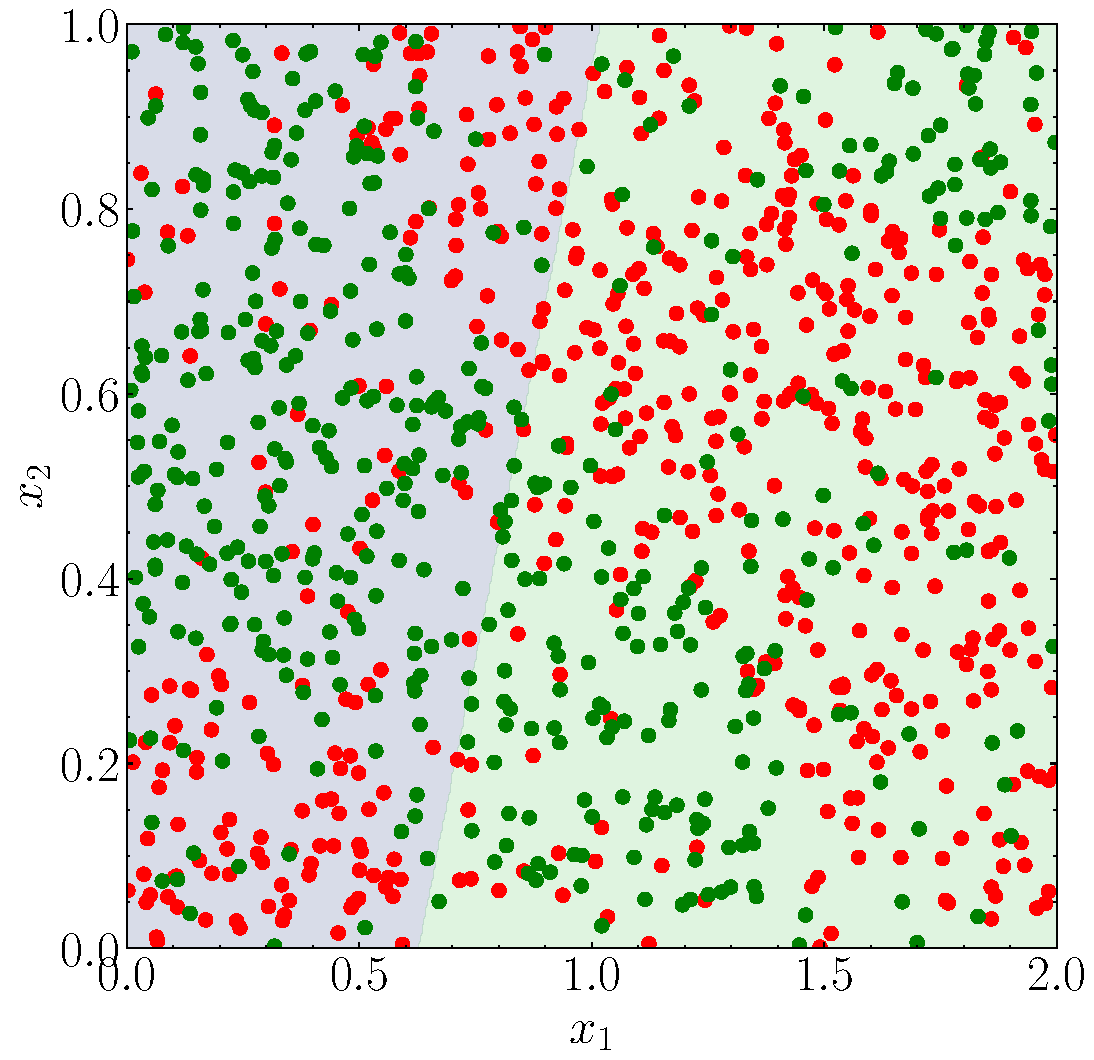
\includegraphics[width=1.5in]{../results/ex1/samples_LOG_dataset_noise20_size_2000}}

\caption{Logistic regression on 2D data with $20\%$ label noise.}
\label{fig:LOG_ex1_noise20}
\end{figure}

\begin{figure}
\centering
\subfigure[Poly, Size $500$]{\label{fig:a}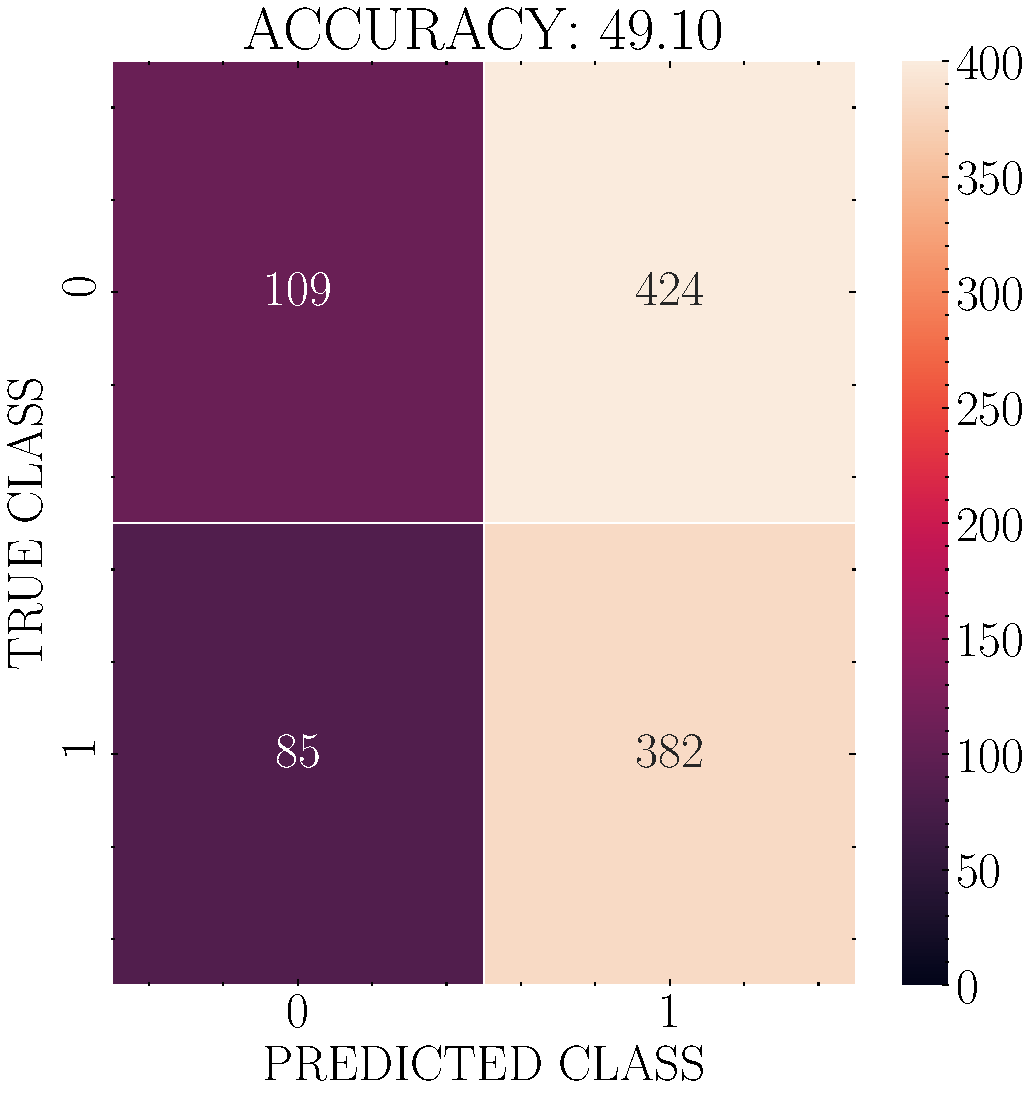
\includegraphics[width=1.5in]{../results/ex1/accuracy_SVM_dataset_noise40_method_poly_size_500}}
\subfigure[SVM-Poly, Classifier]{\label{fig:a}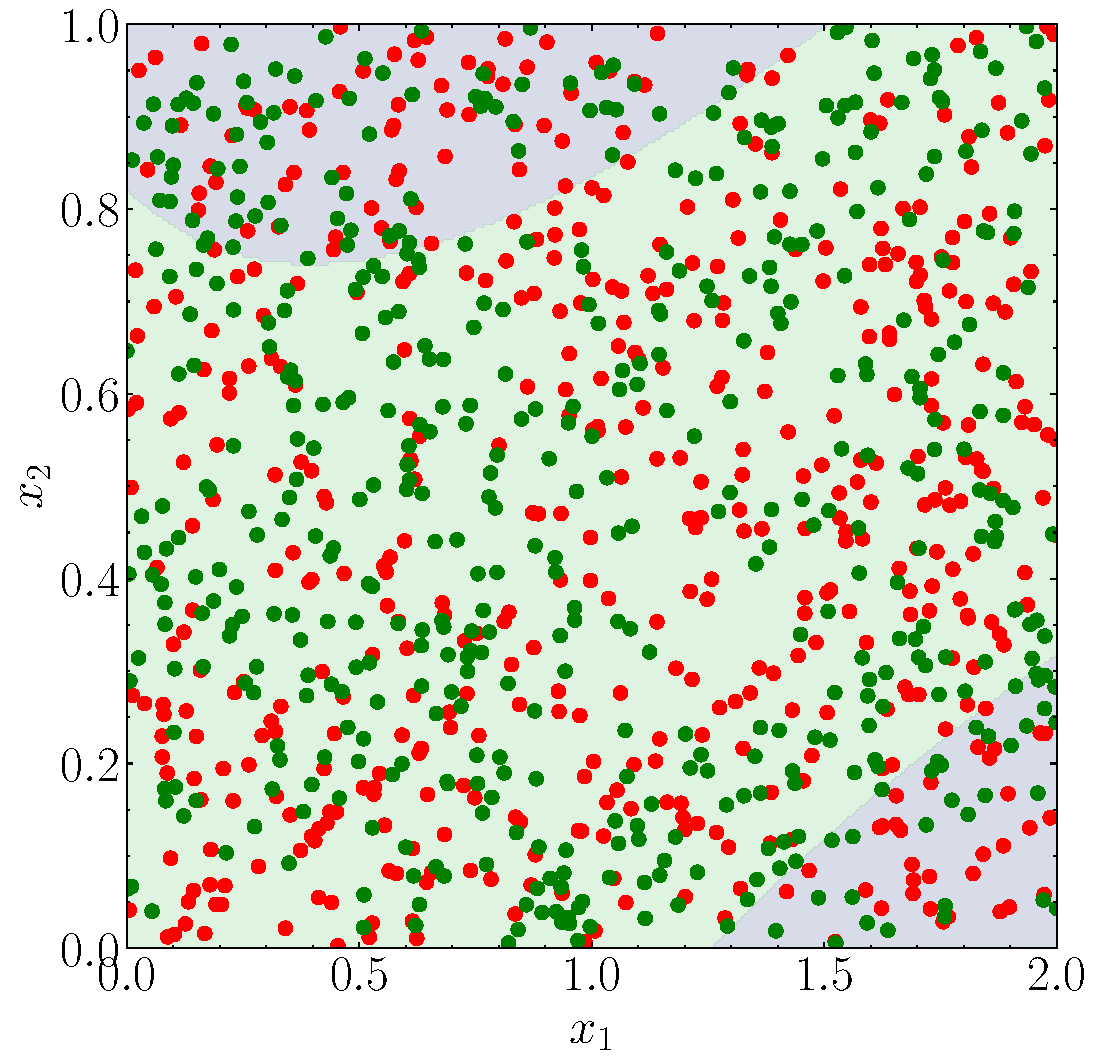
\includegraphics[width=1.5in]{../results/ex1/samples_SVM_dataset_noise40_method_poly_size_500}}
\subfigure[RBF, Size $500$]{\label{fig:a}\includegraphics[width=1.5in]{../results/ex1/accuracy_SVM_dataset_noise40_method_rbf_size_500}}
\subfigure[SVM-RBF Classifier]{\label{fig:a}\includegraphics[width=1.5in]{../results/ex1/samples_SVM_dataset_noise40_method_rbf_size_500}}

\subfigure[Poly, Size $1000$]{\label{fig:a}\includegraphics[width=1.5in]{../results/ex1/accuracy_SVM_dataset_noise40_method_poly_size_1000}}
\subfigure[SVM-Poly, Classifier]{\label{fig:a}\includegraphics[width=1.5in]{../results/ex1/samples_SVM_dataset_noise40_method_poly_size_1000}}
\subfigure[RBF, Size $1000$]{\label{fig:a}\includegraphics[width=1.5in]{../results/ex1/accuracy_SVM_dataset_noise40_method_rbf_size_1000}}
\subfigure[SVM-RBF Classifier]{\label{fig:a}\includegraphics[width=1.5in]{../results/ex1/samples_SVM_dataset_noise40_method_rbf_size_1000}}

\subfigure[Poly, Size $1500$]{\label{fig:a}\includegraphics[width=1.5in]{../results/ex1/accuracy_SVM_dataset_noise40_method_poly_size_1500}}
\subfigure[SVM-Poly, Classifier]{\label{fig:a}\includegraphics[width=1.5in]{../results/ex1/samples_SVM_dataset_noise40_method_poly_size_1500}}
\subfigure[RBF, Size $1500$]{\label{fig:a}\includegraphics[width=1.5in]{../results/ex1/accuracy_SVM_dataset_noise40_method_rbf_size_1500}}
\subfigure[SVM-RBF Classifier]{\label{fig:a}\includegraphics[width=1.5in]{../results/ex1/samples_SVM_dataset_noise40_method_rbf_size_1500}}

\subfigure[Poly, Size $2000$]{\label{fig:a}\includegraphics[width=1.5in]{../results/ex1/accuracy_SVM_dataset_noise40_method_poly_size_2000}}
\subfigure[SVM-Poly, Classifier]{\label{fig:a}\includegraphics[width=1.5in]{../results/ex1/samples_SVM_dataset_noise40_method_poly_size_2000}}
\subfigure[RBF, Size $2000$]{\label{fig:a}\includegraphics[width=1.5in]{../results/ex1/accuracy_SVM_dataset_noise40_method_rbf_size_2000}}
\subfigure[SVM-RBF Classifier]{\label{fig:a}\includegraphics[width=1.5in]{../results/ex1/samples_SVM_dataset_noise40_method_rbf_size_2000}}

\caption{Support vector machines with polynomial kernel of degree $3$ and Gaussian kernel on 2D data with $40\%$ label noise.}
\label{fig:SVM_ex1_noise40}
\end{figure}

\begin{figure}
\centering
\subfigure[Poly, Size $500$]{\label{fig:a}\includegraphics[width=1.5in]{../results/ex1/accuracy_LOG_dataset_noise40_size_500}}
\subfigure[Poly, Size $1000$]{\label{fig:a}\includegraphics[width=1.5in]{../results/ex1/accuracy_LOG_dataset_noise40_size_1000}}
\subfigure[Poly, Size $1500$]{\label{fig:a}\includegraphics[width=1.5in]{../results/ex1/accuracy_LOG_dataset_noise40_size_1500}}
\subfigure[Poly, Size $2000$]{\label{fig:a}\includegraphics[width=1.5in]{../results/ex1/accuracy_LOG_dataset_noise40_size_2000}}

\subfigure[LOG, Classifier]{\label{fig:a}\includegraphics[width=1.5in]{../results/ex1/samples_LOG_dataset_noise40_size_500}}
\subfigure[LOG, Classifier]{\label{fig:a}\includegraphics[width=1.5in]{../results/ex1/samples_LOG_dataset_noise40_size_1000}}
\subfigure[LOG, Classifier]{\label{fig:a}\includegraphics[width=1.5in]{../results/ex1/samples_LOG_dataset_noise40_size_1500}}
\subfigure[LOG, Classifier]{\label{fig:a}\includegraphics[width=1.5in]{../results/ex1/samples_LOG_dataset_noise40_size_2000}}

\caption{Logistic regression on 2D data with $40\%$ label noise.}
\label{fig:LOG_ex1_noise40}
\end{figure}

% ------------------------------------------------------------------------------------------------------------------------------------------------------
% ------------------------------------------------------------------------------------------------------------------------------------------------------

\section{Neural Network for Classification on 2D Board Data}
\label{sec:nn_board}

\begin{figure}
\centering
\subfigure[SGD, Size $2000$]{\label{fig:a}\includegraphics[width=1.5in]{../results/ex2/accuracy_NN_dataset_Board0_size_2000_method_SGD}}
\subfigure[SGD Classifier]{\label{fig:a}\includegraphics[width=1.5in]{../results/ex2/samples_NN_dataset_Board0_size_2000_method_SGD}}
\subfigure[Adam, Size $2000$]{\label{fig:a}\includegraphics[width=1.5in]{../results/ex2/accuracy_NN_dataset_Board0_size_2000_method_Adam}}
\subfigure[Adam Classifier]{\label{fig:a}\includegraphics[width=1.5in]{../results/ex2/samples_NN_dataset_Board0_size_2000_method_Adam}}
%\subfigure[SGD Loss Function]{\label{fig:a}\includegraphics[width=1.5in]{../results/ex2/loss_NN_dataset_Board0_size_2000_method_SGD}}
%\subfigure[Adam Loss Function]{\label{fig:a}\includegraphics[width=1.5in]{../results/ex2/loss_NN_dataset_Board0_size_2000_method_Adam}}

\subfigure[SGD, Size $3000$]{\label{fig:a}\includegraphics[width=1.5in]{../results/ex2/accuracy_NN_dataset_Board0_size_3000_method_SGD}}
\subfigure[SGD Classifier]{\label{fig:a}\includegraphics[width=1.5in]{../results/ex2/samples_NN_dataset_Board0_size_3000_method_SGD}}
\subfigure[Adam, Size $3000$]{\label{fig:a}\includegraphics[width=1.5in]{../results/ex2/accuracy_NN_dataset_Board0_size_3000_method_Adam}}
\subfigure[Adam Classifier]{\label{fig:a}\includegraphics[width=1.5in]{../results/ex2/samples_NN_dataset_Board0_size_3000_method_Adam}}
%\subfigure[SGD Loss Function]{\label{fig:a}\includegraphics[width=1.5in]{../results/ex2/loss_NN_dataset_Board0_size_3000_method_SGD}}
%\subfigure[Adam Loss Function]{\label{fig:a}\includegraphics[width=1.5in]{../results/ex2/loss_NN_dataset_Board0_size_3000_method_Adam}}

\subfigure[SGD, Size $4000$]{\label{fig:a}\includegraphics[width=1.5in]{../results/ex2/accuracy_NN_dataset_Board0_size_4000_method_SGD}}
\subfigure[SGD Classifier]{\label{fig:a}\includegraphics[width=1.5in]{../results/ex2/samples_NN_dataset_Board0_size_4000_method_SGD}}
\subfigure[Adam, Size $4000$]{\label{fig:a}\includegraphics[width=1.5in]{../results/ex2/accuracy_NN_dataset_Board0_size_4000_method_Adam}}
\subfigure[Adam Classifier]{\label{fig:a}\includegraphics[width=1.5in]{../results/ex2/samples_NN_dataset_Board0_size_4000_method_Adam}}
%\subfigure[SGD Loss Function]{\label{fig:a}\includegraphics[width=1.5in]{../results/ex2/loss_NN_dataset_Board0_size_4000_method_SGD}}
%\subfigure[Adam Loss Function]{\label{fig:a}\includegraphics[width=1.5in]{../results/ex2/loss_NN_dataset_Board0_size_4000_method_Adam}}

\subfigure[SVM, Size $2000$]{\label{fig:a}\includegraphics[width=1.5in]{../results/ex2/accuracy_SVM_dataset_Board0_size_2000}}
\subfigure[SVM, Size $3000$]{\label{fig:a}\includegraphics[width=1.5in]{../results/ex2/accuracy_SVM_dataset_Board0_size_3000}}
\subfigure[SVM, Size $4000$]{\label{fig:a}\includegraphics[width=1.5in]{../results/ex2/accuracy_SVM_dataset_Board0_size_4000}}

\caption{Feedforward network on 2D data with no label noise.}
\label{fig:NN_ex2_board0}
\end{figure}

\begin{figure}
\centering
\subfigure[SGD, Size $2000$]{\label{fig:a}\includegraphics[width=1.5in]{../results/ex2/accuracy_NN_dataset_Board10_size_2000_method_SGD}}
\subfigure[SGD Classifier]{\label{fig:a}\includegraphics[width=1.5in]{../results/ex2/samples_NN_dataset_Board10_size_2000_method_SGD}}
\subfigure[Adam, Size $2000$]{\label{fig:a}\includegraphics[width=1.5in]{../results/ex2/accuracy_NN_dataset_Board10_size_2000_method_Adam}}
\subfigure[Adam Classifier]{\label{fig:a}\includegraphics[width=1.5in]{../results/ex2/samples_NN_dataset_Board10_size_2000_method_Adam}}
%\subfigure[SGD Loss Function]{\label{fig:a}\includegraphics[width=1.5in]{../results/ex2/loss_NN_dataset_Board10_size_2000_method_SGD}}
%\subfigure[Adam Loss Function]{\label{fig:a}\includegraphics[width=1.5in]{../results/ex2/loss_NN_dataset_Board10_size_2000_method_Adam}}

\subfigure[SGD, Size $3000$]{\label{fig:a}\includegraphics[width=1.5in]{../results/ex2/accuracy_NN_dataset_Board10_size_3000_method_SGD}}
\subfigure[SGD Classifier]{\label{fig:a}\includegraphics[width=1.5in]{../results/ex2/samples_NN_dataset_Board10_size_3000_method_SGD}}
\subfigure[Adam, Size $3000$]{\label{fig:a}\includegraphics[width=1.5in]{../results/ex2/accuracy_NN_dataset_Board10_size_3000_method_Adam}}
\subfigure[Adam Classifier]{\label{fig:a}\includegraphics[width=1.5in]{../results/ex2/samples_NN_dataset_Board10_size_3000_method_Adam}}
%\subfigure[SGD Loss Function]{\label{fig:a}\includegraphics[width=1.5in]{../results/ex2/loss_NN_dataset_Board10_size_3000_method_SGD}}
%\subfigure[Adam Loss Function]{\label{fig:a}\includegraphics[width=1.5in]{../results/ex2/loss_NN_dataset_Board10_size_3000_method_Adam}}

\subfigure[SGD, Size $4000$]{\label{fig:a}\includegraphics[width=1.5in]{../results/ex2/accuracy_NN_dataset_Board10_size_4000_method_SGD}}
\subfigure[SGD Classifier]{\label{fig:a}\includegraphics[width=1.5in]{../results/ex2/samples_NN_dataset_Board10_size_4000_method_SGD}}
\subfigure[Adam, Size $4000$]{\label{fig:a}\includegraphics[width=1.5in]{../results/ex2/accuracy_NN_dataset_Board10_size_4000_method_Adam}}
\subfigure[Adam Classifier]{\label{fig:a}\includegraphics[width=1.5in]{../results/ex2/samples_NN_dataset_Board10_size_4000_method_Adam}}
%\subfigure[SGD Loss Function]{\label{fig:a}\includegraphics[width=1.5in]{../results/ex2/loss_NN_dataset_Board10_size_4000_method_SGD}}
%\subfigure[Adam Loss Function]{\label{fig:a}\includegraphics[width=1.5in]{../results/ex2/loss_NN_dataset_Board10_size_4000_method_Adam}}

\subfigure[SVM, Size $2000$]{\label{fig:a}\includegraphics[width=1.5in]{../results/ex2/accuracy_SVM_dataset_Board10_size_2000}}
\subfigure[SVM, Size $3000$]{\label{fig:a}\includegraphics[width=1.5in]{../results/ex2/accuracy_SVM_dataset_Board10_size_3000}}
\subfigure[SVM, Size $4000$]{\label{fig:a}\includegraphics[width=1.5in]{../results/ex2/accuracy_SVM_dataset_Board10_size_4000}}

\caption{Feedforward network on 2D data with $10\%$ label noise.}
\label{fig:NN_ex2_Board10}
\end{figure}

\begin{figure}
\centering
\subfigure[SGD, Size $2000$]{\label{fig:a}\includegraphics[width=1.5in]{../results/ex2/accuracy_NN_dataset_Board25_size_2000_method_SGD}}
\subfigure[SGD Classifier]{\label{fig:a}\includegraphics[width=1.5in]{../results/ex2/samples_NN_dataset_Board25_size_2000_method_SGD}}
\subfigure[Adam, Size $2000$]{\label{fig:a}\includegraphics[width=1.5in]{../results/ex2/accuracy_NN_dataset_Board25_size_2000_method_Adam}}
\subfigure[Adam Classifier]{\label{fig:a}\includegraphics[width=1.5in]{../results/ex2/samples_NN_dataset_Board25_size_2000_method_Adam}}
%\subfigure[SGD Loss Function]{\label{fig:a}\includegraphics[width=1.5in]{../results/ex2/loss_NN_dataset_Board25_size_2000_method_SGD}}
%\subfigure[Adam Loss Function]{\label{fig:a}\includegraphics[width=1.5in]{../results/ex2/loss_NN_dataset_Board25_size_2000_method_Adam}}

\subfigure[SGD, Size $3000$]{\label{fig:a}\includegraphics[width=1.5in]{../results/ex2/accuracy_NN_dataset_Board25_size_3000_method_SGD}}
\subfigure[SGD Classifier]{\label{fig:a}\includegraphics[width=1.5in]{../results/ex2/samples_NN_dataset_Board25_size_3000_method_SGD}}
\subfigure[Adam, Size $3000$]{\label{fig:a}\includegraphics[width=1.5in]{../results/ex2/accuracy_NN_dataset_Board25_size_3000_method_Adam}}
\subfigure[Adam Classifier]{\label{fig:a}\includegraphics[width=1.5in]{../results/ex2/samples_NN_dataset_Board25_size_3000_method_Adam}}
%\subfigure[SGD Loss Function]{\label{fig:a}\includegraphics[width=1.5in]{../results/ex2/loss_NN_dataset_Board25_size_3000_method_SGD}}
%\subfigure[Adam Loss Function]{\label{fig:a}\includegraphics[width=1.5in]{../results/ex2/loss_NN_dataset_Board25_size_3000_method_Adam}}

\subfigure[SGD, Size $4000$]{\label{fig:a}\includegraphics[width=1.5in]{../results/ex2/accuracy_NN_dataset_Board25_size_4000_method_SGD}}
\subfigure[SGD Classifier]{\label{fig:a}\includegraphics[width=1.5in]{../results/ex2/samples_NN_dataset_Board25_size_4000_method_SGD}}
\subfigure[Adam, Size $4000$]{\label{fig:a}\includegraphics[width=1.5in]{../results/ex2/accuracy_NN_dataset_Board25_size_4000_method_Adam}}
\subfigure[Adam Classifier]{\label{fig:a}\includegraphics[width=1.5in]{../results/ex2/samples_NN_dataset_Board25_size_4000_method_Adam}}
%\subfigure[SGD Loss Function]{\label{fig:a}\includegraphics[width=1.5in]{../results/ex2/loss_NN_dataset_Board25_size_4000_method_SGD}}
%\subfigure[Adam Loss Function]{\label{fig:a}\includegraphics[width=1.5in]{../results/ex2/loss_NN_dataset_Board25_size_4000_method_Adam}}

\subfigure[SVM, Size $2000$]{\label{fig:a}\includegraphics[width=1.5in]{../results/ex2/accuracy_SVM_dataset_Board25_size_2000}}
\subfigure[SVM, Size $3000$]{\label{fig:a}\includegraphics[width=1.5in]{../results/ex2/accuracy_SVM_dataset_Board25_size_3000}}
\subfigure[SVM, Size $4000$]{\label{fig:a}\includegraphics[width=1.5in]{../results/ex2/accuracy_SVM_dataset_Board25_size_4000}}

\caption{Feedforward network on 2D data with $25\%$ label noise.}
\label{fig:NN_ex2_Board25}
\end{figure}

% ------------------------------------------------------------------------------------------------------------------------------------------------------
% ------------------------------------------------------------------------------------------------------------------------------------------------------

\section{Convolutional Network for Classification on MNIST}
\label{sec:nn_mnist}

\begin{figure}
\centering
\subfigure[CNN with Adam]{\label{fig:a}\includegraphics[width=2in]{../results/ex3/accuracy_CNN_dataset_MNIST_method_Adam}}
\subfigure[CNN Loss Function]{\label{fig:a}\includegraphics[width=2in]{../results/ex3/loss_CNN_dataset_MNIST_method_Adam}}
\subfigure[SVM with RBF Kernel]{\label{fig:a}\includegraphics[width=2in]{../results/ex3/accuracy_SVM_dataset_mnist}}
\caption{Convolutional neural network and support vector machines for MNIST classification.}
\label{fig:CNN_ex3_MNIST}
\end{figure}

\begin{figure}
\centering
\subfigure[CNN with Adam]{\label{fig:a}\includegraphics[width=2in]{../results/ex3/accuracy_CNN_dataset_mnist-rot_method_Adam}}
\subfigure[CNN Loss Function]{\label{fig:a}\includegraphics[width=2in]{../results/ex3/loss_CNN_dataset_mnist-rot_method_Adam}}
\subfigure[SVM with RBF Kernel]{\label{fig:a}\includegraphics[width=2in]{../results/ex3/accuracy_SVM_dataset_mnist-rot}}
\caption{Convolutional neural network and support vector machines for MNIST-ROT classification.}
\label{fig:CNN_ex3_MNIST-ROT}
\end{figure}

% ------------------------------------------------------------------------------------------------------------------------------------------------------
% ------------------------------------------------------------------------------------------------------------------------------------------------------

\section{Convolutional Network for Classification on MNIST}
\label{sec:nn_mnist}

% ------------------------------------------------------------------------------------------------------------------------------------------------------
% ------------------------------------------------------------------------------------------------------------------------------------------------------


\section{Code Repository}
The Python codes to reproduce the results can be found in the GitHub repository \url{https://github.com/kamath-abhijith/Nonlinear_Models}. Use \texttt{requirements.txt} to install the dependencies and the shell scripts to generate the figures.


\end{document} 
